\chapter{Implementation}
\label{chap:implementation}

This section describes the artefact development process. Despite multiple stumbling blocks during development, these were overcome through problem-solving, thorough investigation and reading of software documentation.  

\section{Development Environment}
\label{implementation:de}

Visual Studio Code (VSCode) was chosen as the development environment (\cite{noauthor_visual_nodate}). VSCode was chosen due to its flexibility in working with multiple programming languages through the use of extensions. The React.js Framework, JavaScript and Go Language extensions were installed to ensure seamless development of the back and front end. The ESLint extension was also used to ensure the consistency and readability of the codebase.

\section{Iteration 1 - Basic UI and Core Routing}
\label{implementation:iteration1}
The initial stages of development began using a first draft of elicited requirements \see{appendix:initial-user-requirements} where later on, a new set of user requirements was formed based on primary research. This method proved effective in not delaying initial development, where the core requirements were unlikely to change greatly. Furthermore, Iteration 1 (i1) consisted of implementing the building blocks of the artefact, including setting up a React.js App, web server, database and core routing functionalities.

\subsection{Leaflet - Open Street Map (OSM)}
\label{iteration1:leaflet-osm}
The Map component was developed first because other components would be dependent on its functionality. The component contained a div element containing the MapContainer component imported from React Leaflet (\cite{noauthor_react_nodate}). The component includes a tile layer to make API requests to OSM (\cite{noauthor_openstreetmap_nodate}) to retrieve the tile images for the map. Temporary variables were set up to store the latitude and longitude values representing the start and end of a route, then drawn on the map using a polyline and marker points \see{fig:basic-map-with-route}. 

\begin{figure}[!ht]
    \centering
    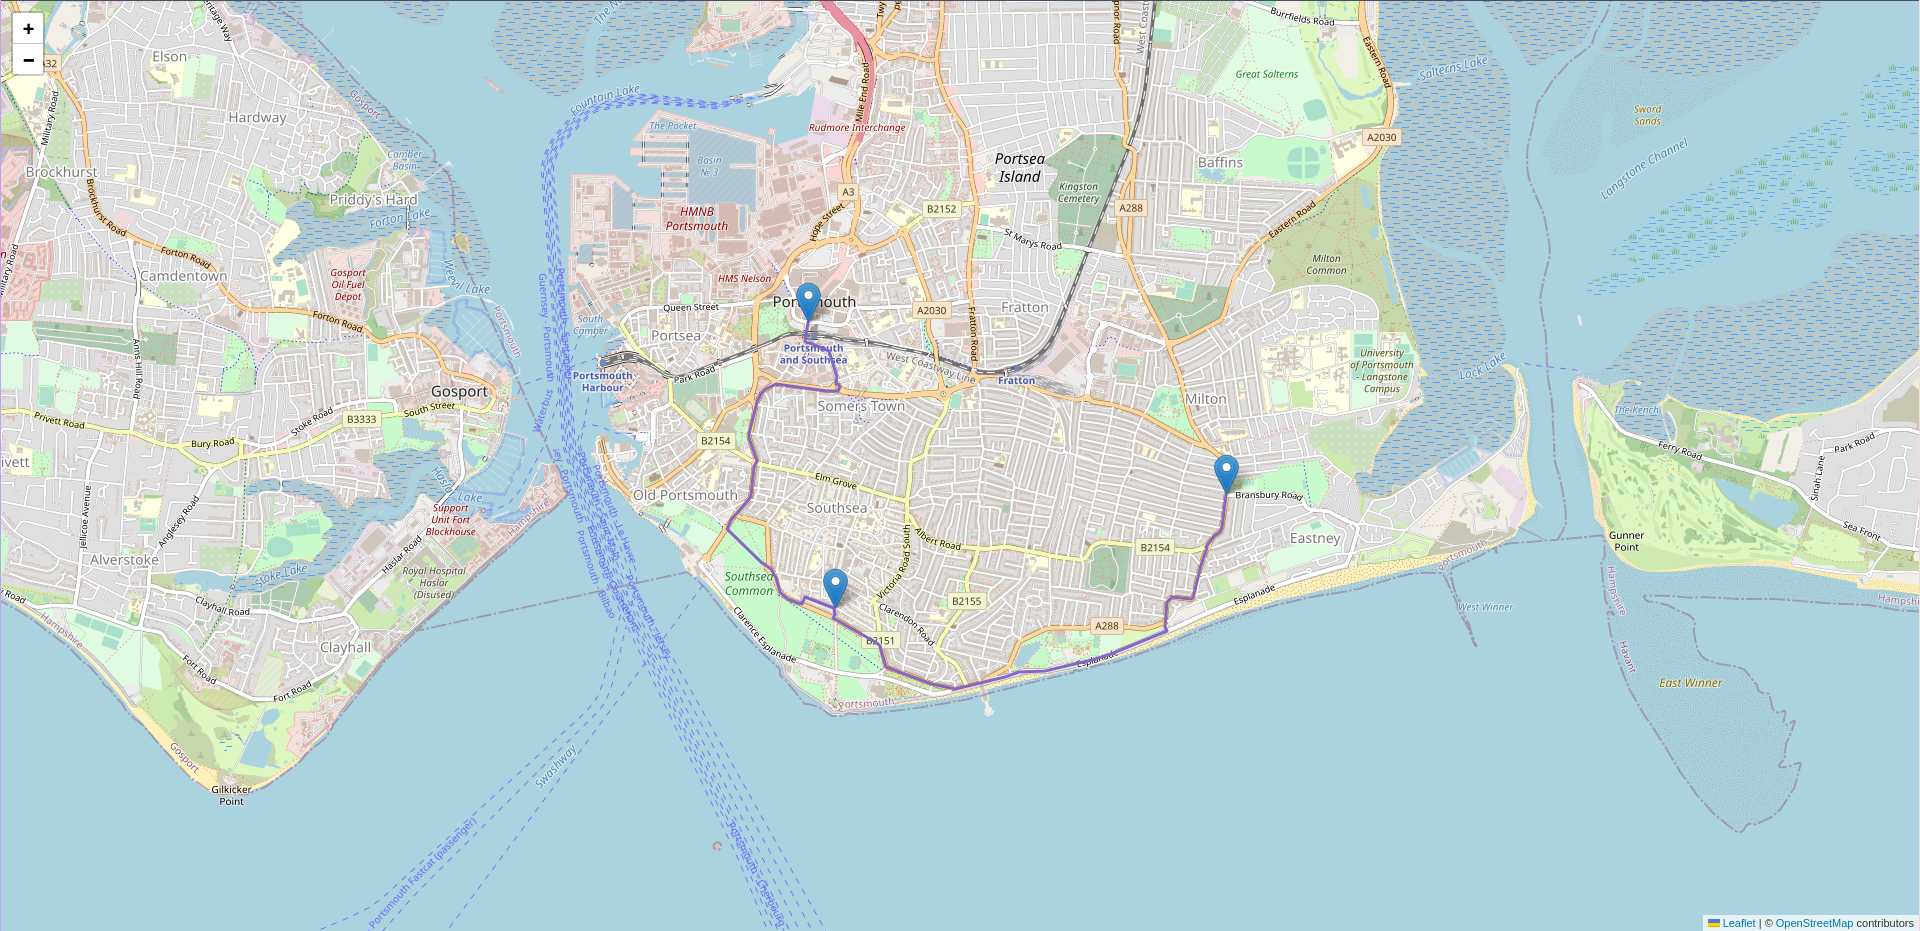
\includegraphics[width=425px]{figures/Progress Images/Iteration-1/SR25/Basic Route.png}
    \caption{Basic Map with Route}
    \label{fig:basic-map-with-route}
\end{figure}

\subsection{Basic Route Planning}
\label{iteration1:basic-routing}
After conducting research, the most effective way to implement route planning with Leaflet was to use Leaflet Routing Machine (\cite{noauthor_leaflet_nodate-1}). This library enabled a RoutingMachine component to be added on top of the Map component, providing a basic, customisable route planning UI \see{fig:routing-ui}. The routing API in use at the beginning was Open Source Routing Machine (OSRM) (\cite{noauthor_project_nodate}) which appeared to meet all requirements of a routing algorithm until round trip routing was required \see{iteration3:round-trip}. This new routing functionality planned a route from the user's start, destination and any intermediate locations. At this stage, the route could be altered through the use of waypoints, but the artefact did not provide any further custom routing features to the user.
\begin{figure}[!ht]
    \centering
    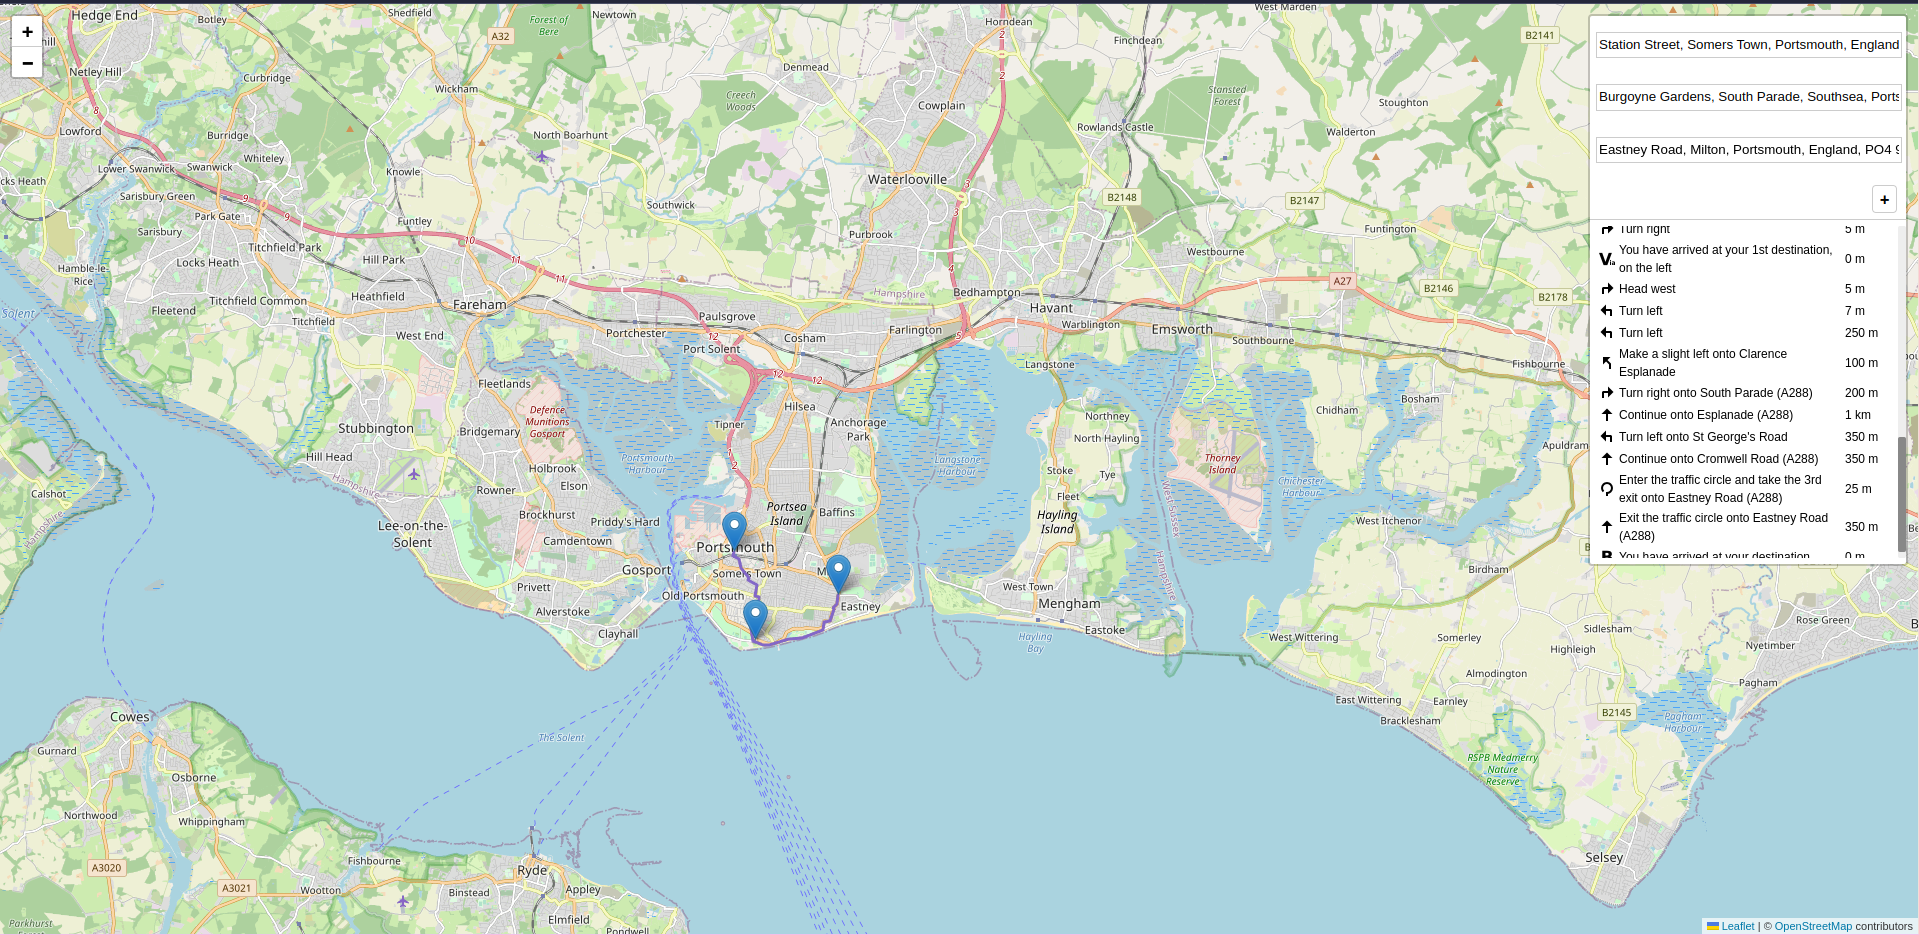
\includegraphics[width=425px]{figures/Progress Images/Iteration-1/SR1/Basic Destination Overlay Set up.png}
    \caption{Routing UI}
    \label{fig:routing-ui}
  \end{figure}

\subsection{Elevation Chart}
\label{iteration1:elevation-chart}
Chart.js was used to create the ElevationChart component (\cite{noauthor_chartjs_nodate}). A div was created to hold the chart component, where the elevation data was gathered from a state variable called 'coordinates' which contained the route latitude, longitude, and the elevation for each coordinate \see{fig:waypoint-arr}. The distance along the route for each elevation point was calculated by dividing the total route distance ('summary.totalDistance' variable) by the length of the 'coordinates' array. To ensure continuity between the map and the elevation plot, a simple feature was added to allow the user to hover over the elevation plot, with the matching point along the route being highlighted. The canvas hover point was found and matched with the corresponding latitude and longitude point used to draw a circle element on the Leaflet map \see{fig:elevation-hover}.

\begin{figure}[!ht]
    \centering
    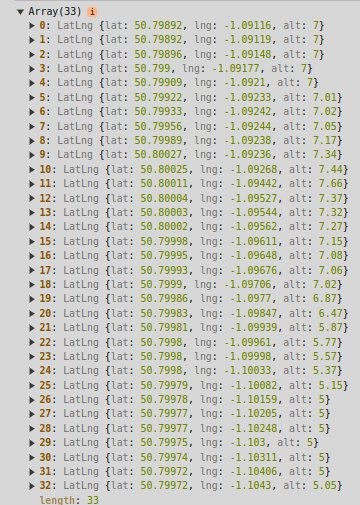
\includegraphics[width=200px]{figures/Progress Images/Iteration-1/SR1/waypoint-arr.png}
    \caption{Route Waypoint/Elevation Array}
    \label{fig:waypoint-arr}
  \end{figure}

\begin{figure}[!ht]
    \centering
    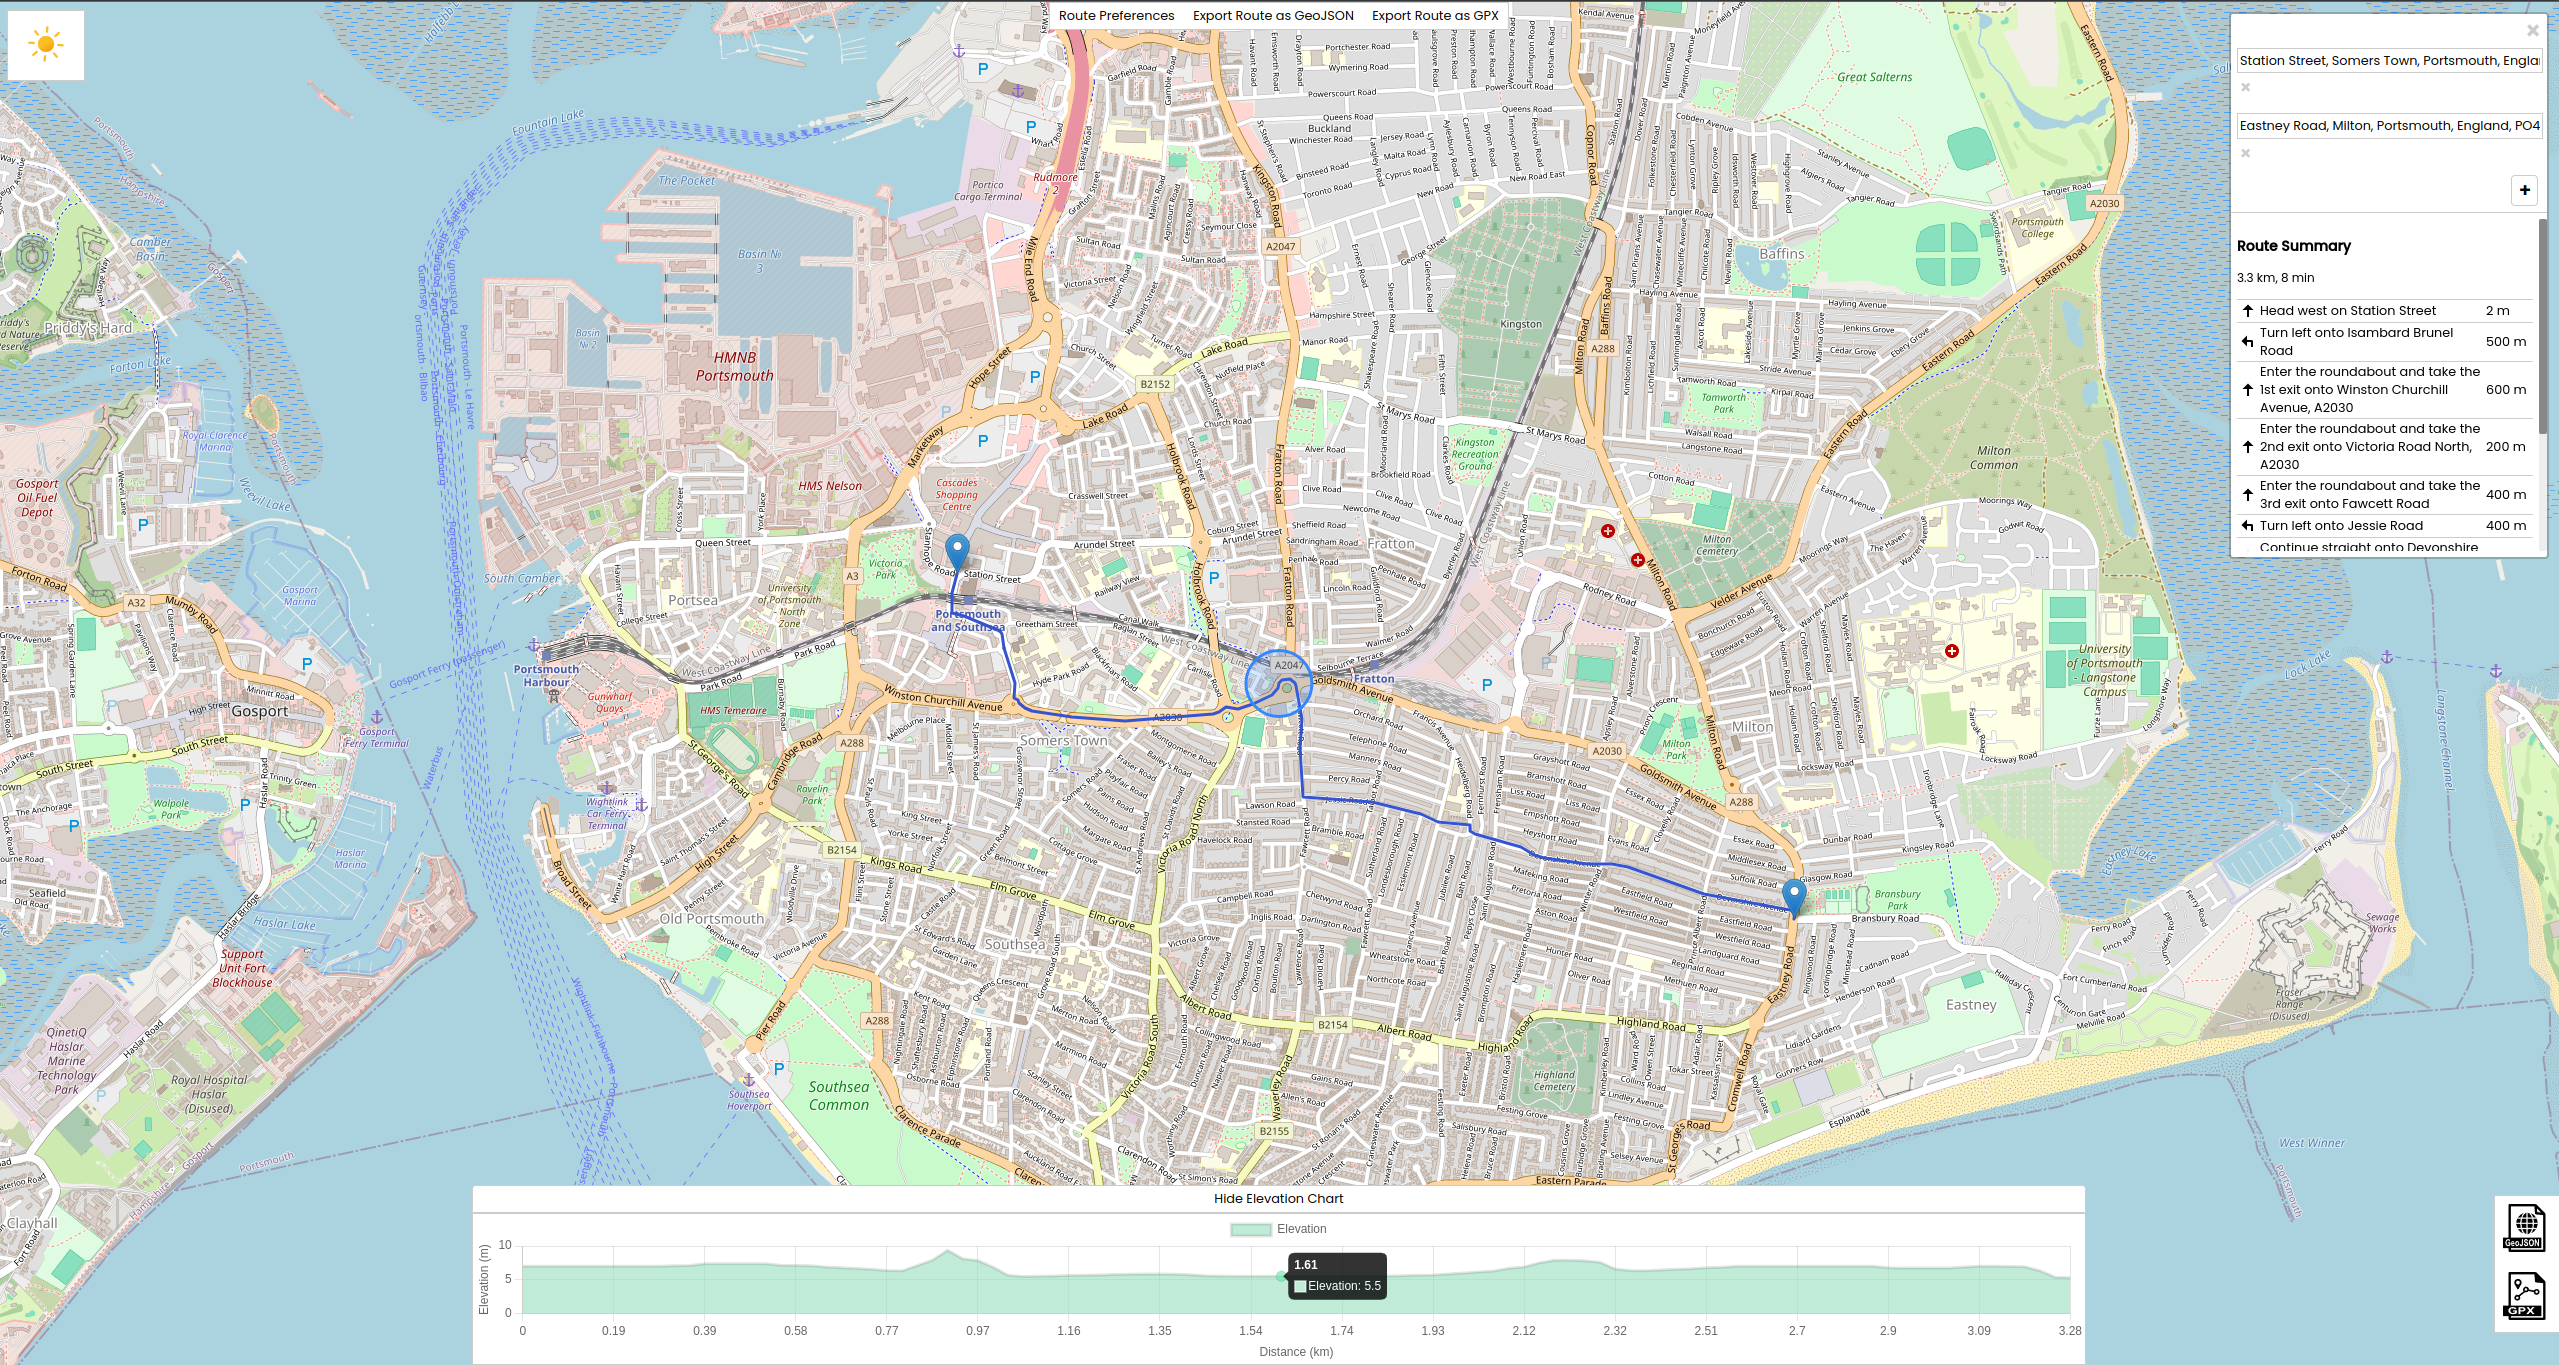
\includegraphics[width=425px]{figures/Progress Images/Iteration-1/SR28/elevation-hover.png}
    \caption{Elevation Plot Hover Functionality}
    \label{fig:elevation-hover}
\end{figure}

\subsection{Weather Information Panel}
\label{iteration1:weather-panel}
A weather panel was created within i1, displaying weather information for the current day at the user's location. The weather panel used the geolocation API called within a React useEffect to get the user's approximate location, asking for permission via a pop-up window, then storing the geolocation in a state variable. The coordinates returned from the API were then passed to Open Weather Map to gather all weather data for the current day. The Meteocons icons (\cite{noauthor_weather_nodate}) were used to display images demonstrating the current weather conditions \see{fig:basic-weather-panel}. The visibility of the weather panel was determined by a State variable, if the variable was true, the size of the panel expanded, and when false, reduced.

\begin{figure}[!ht]
    \centering
    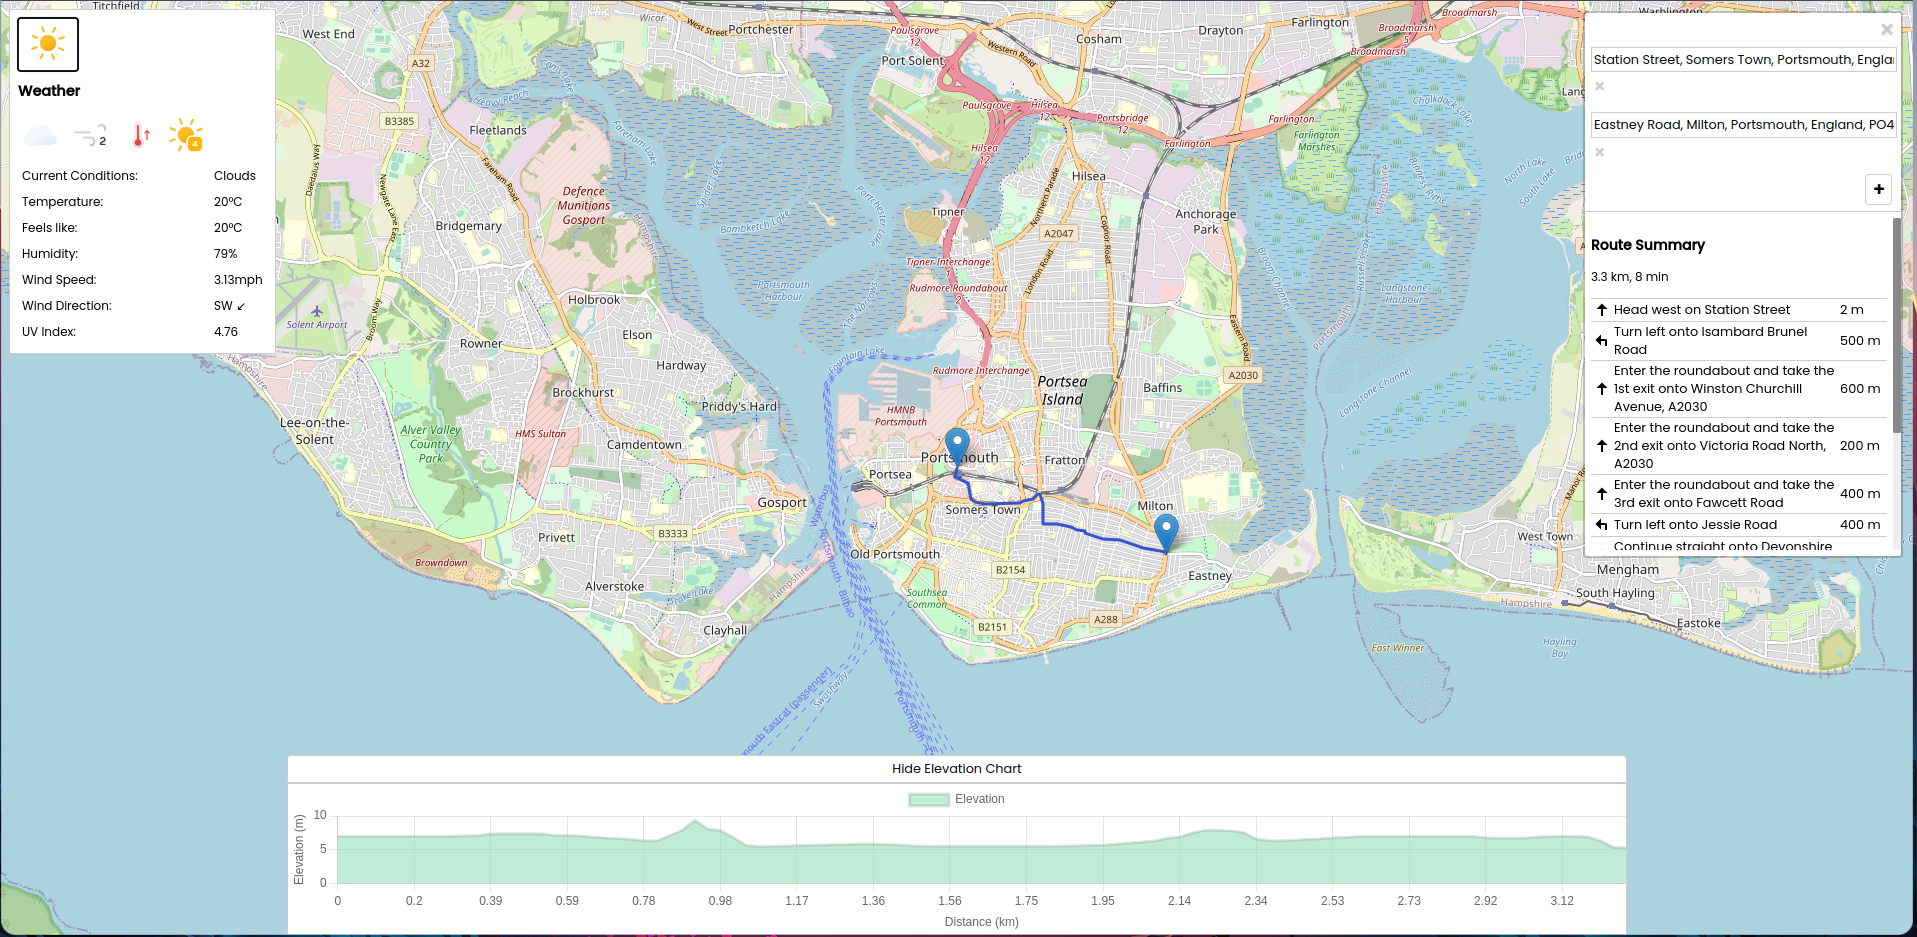
\includegraphics[width=300px]{figures/Progress Images/Iteration-1/SR19&SR28 Combined/SR19&SR28 Merged.png}
    \caption{Weather Panel}
    \label{fig:basic-weather-panel}
\end{figure}

\subsection{Main Challenges}
\label{iteration1:main-challenges}
The main challenge of i1, was integrating multiple services to communicate seamlessly through the React.js frontend. Syncing hovering over the elevation plot, with a matching point along the route polyline, also proved difficult. Despite the calculations being simple to determine at what latitude and longitude to draw the circle marker on the map when hovering on the plot, getting the map instance reference was more difficult than expected. Initially, the reference would return undefined, therefore no marker was drawn on the map, however after implementing a useState and declaring a copy of the map instance, the hover functionality worked seamlessly.

Furthermore, the only other challenge faced was retrieving the user's geolocation from the browser. A useEffect was required to access the geolocation API, however, the useState was at first missed to store the geolocation value after the data was returned. Once the state variable was added, the weather panel would re-render once the data was retrieved.

\section{Iteration 2 - Route Sharing, Hazard Index and POI Integration}
\label{implementation:iteration2}

Unlike i1, Iteration 2 (i2) development was conducted after the primary research and requirements review had been completed. The remaining updated requirements were prioritised and distributed between i2 and Iteration 3 (i3) \see{implementation:iteration3}. I2 builds on i1, enhancing existing functionality and introducing new features. 

\subsection{Sharing Route Functionality}
\label{iteration2:sharing-route}

Route sharing was implemented with i2, when routes were found using OpenRouteService (ORS), GPX (\cite{noauthor_gpx_nodate}) and GeoJSON (\cite{noauthor_geojson_nodate}) strings were generated. These were then used to create a share-to-email feature using the Twilio SENDGRID API (\cite{noauthor_email_nodate}). Initially, it was planned to send emails directly to SENDGRID from the client. However, it was found that SENDGRID only accepts incoming requests from the server. Therefore, an API endpoint was created with Gin to handle the POST request from the front end. 

Each email would contain a simple amount of text with the included GPX and/or GeoJSON files selected for export. A modal was created to display the email form, where the user could input the recipient's email address, and route name and choose what type of file to share \see{fig:basic-weather-panel}.

Initially, it was planned to use the Strava API to upload GPX files directly to the Strava Routes, however, it was found that the Strava API had no such endpoint to integrate with routes. It was decided to still implement Strava integration, but with activities, enabling route export as an activity for users without dedicated fitness devices. 

A modal was created \see{fig:strava-modal} and a POST request endpoint was set up to handle the request to the Strava API. The user authenticate with strava, to enable access to upload activities to their account. Once logged in, the user could select the route to upload, then the artefact would send the GPX file to the Strava API and saved to their account \see{fig:strava-example}.

\begin{figure}[!ht]
  \centering
  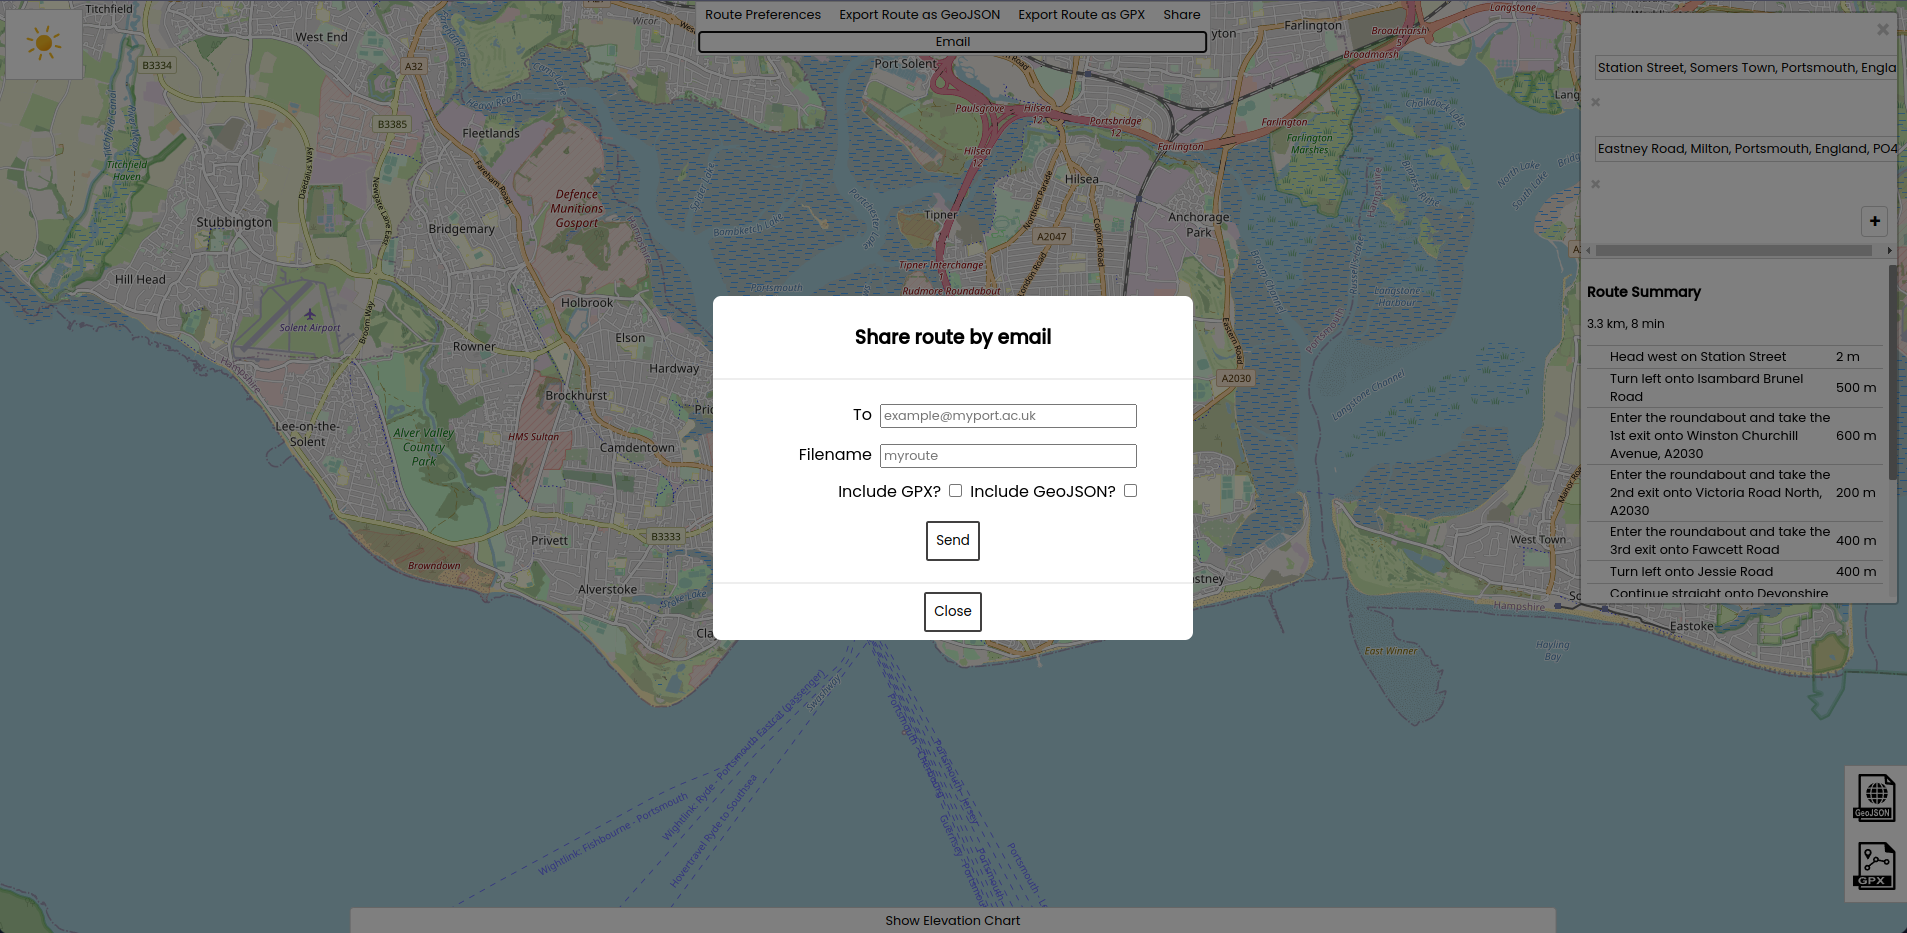
\includegraphics[width=425px]{figures/Progress Images/Iteration-2/SR17/SR17png.png}
  \caption{Share to Email Modal}
  \label{fig:share-email-modal}
\end{figure}

\begin{figure}[!ht]
  \centering
  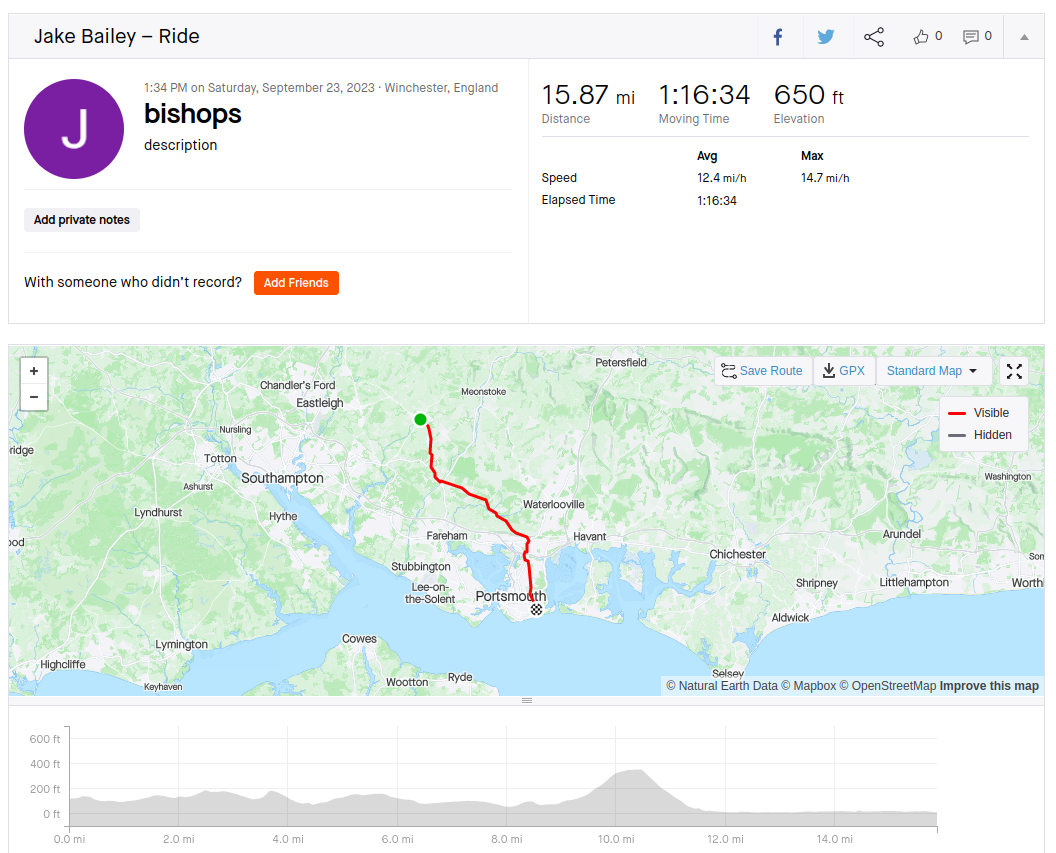
\includegraphics[width=425px]{figures/Progress Images/Iteration-2/SR18/SR18 Upload Example 1.png}
  \caption{Strava Activity}
  \label{fig:strava-example}
\end{figure}

\begin{figure}[!ht]
  \centering
  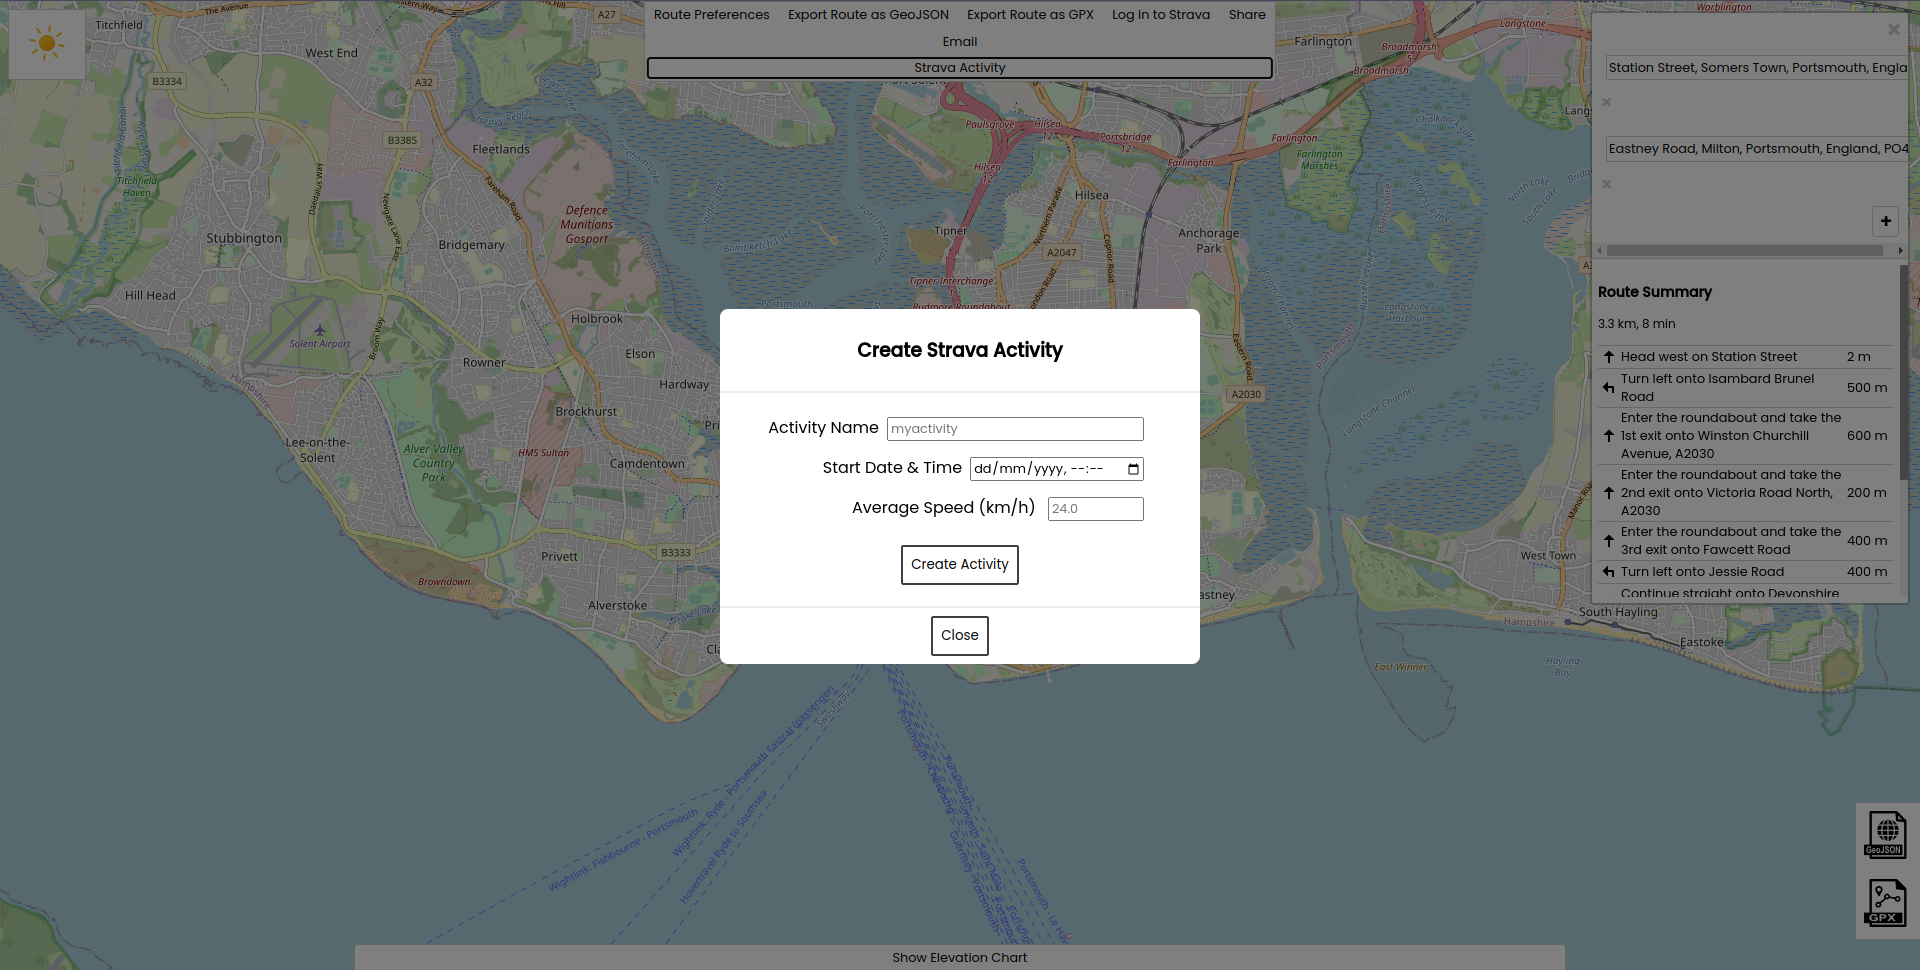
\includegraphics[width=425px]{figures/Progress Images/Iteration-2/SR18/SR18 Strava Modal.png}
  \caption{Share to Strava Modal}
  \label{fig:strava-modal}
\end{figure}


\subsection{Hazard Index Database Creation and Integration}
\label{iteration2:hazard-index}

The hazard index database development was the largest task of i2 and was created using PostgreSQL using PostGIS. The database was split into eight tables representing a hazard, related details and its geospatial data \see{system:database-design}. Hazard types were chosen based on the most relevant hazards defined on the OSM wiki (\cite{noauthor_keyhazard_nodate}) with the addition of a 'Cycling Infrastructure' hazard. The 'Cycling Infrastructure' hazard type was added to allow users to report and view bad cycling infrastructure, with the intention of routing algorithms avoiding these areas in the future \see{evaluation:future}.

To integrate the database into the artefact, API endpoints were created to handle GET and POST requests for the database. The database was connected to the Go backend using the 'lib/pq' package (\cite{noauthor_pq_nodate}), with Gin handling the request routing to the database. Using the fetch API, the frontend could make API calls, to add and retrieve hazards from the database, supplying coordinates for the hazard location/area and the hazard type \see{fig:hazard-creation}.

To enable users to contribute to the hazard index database, a UI was created using the Leaflet Draw API (\cite{noauthor_leaflet_nodate-2}). The API allowed buttons to draw markers and polygons to be added to the map. These buttons were used to create a hazard, where an event handler would catch the polygon/marker-drawn event. This handler function would then proceed to open the hazard creation modal, with the coordinates of the drawn polygon/marker passed to the modal via props. The user could then add the extra information required for the hazard and submit the hazard to the database.

Furthermore, to display the hazard data on the map, a new layer was created. This layer included hazards and cycling infrastructure retrieved from the database. These were shown as both markers and polygons to represent a point or area \see{fig:hazard-layer}. The API endpoint was set up to allow the user to retrieve all hazards within a five-mile radius of a point, therefore, as the map was panned, the hazard layer would update \see{fig:hazard-API}.

\begin{figure}[!ht]
  \centering
  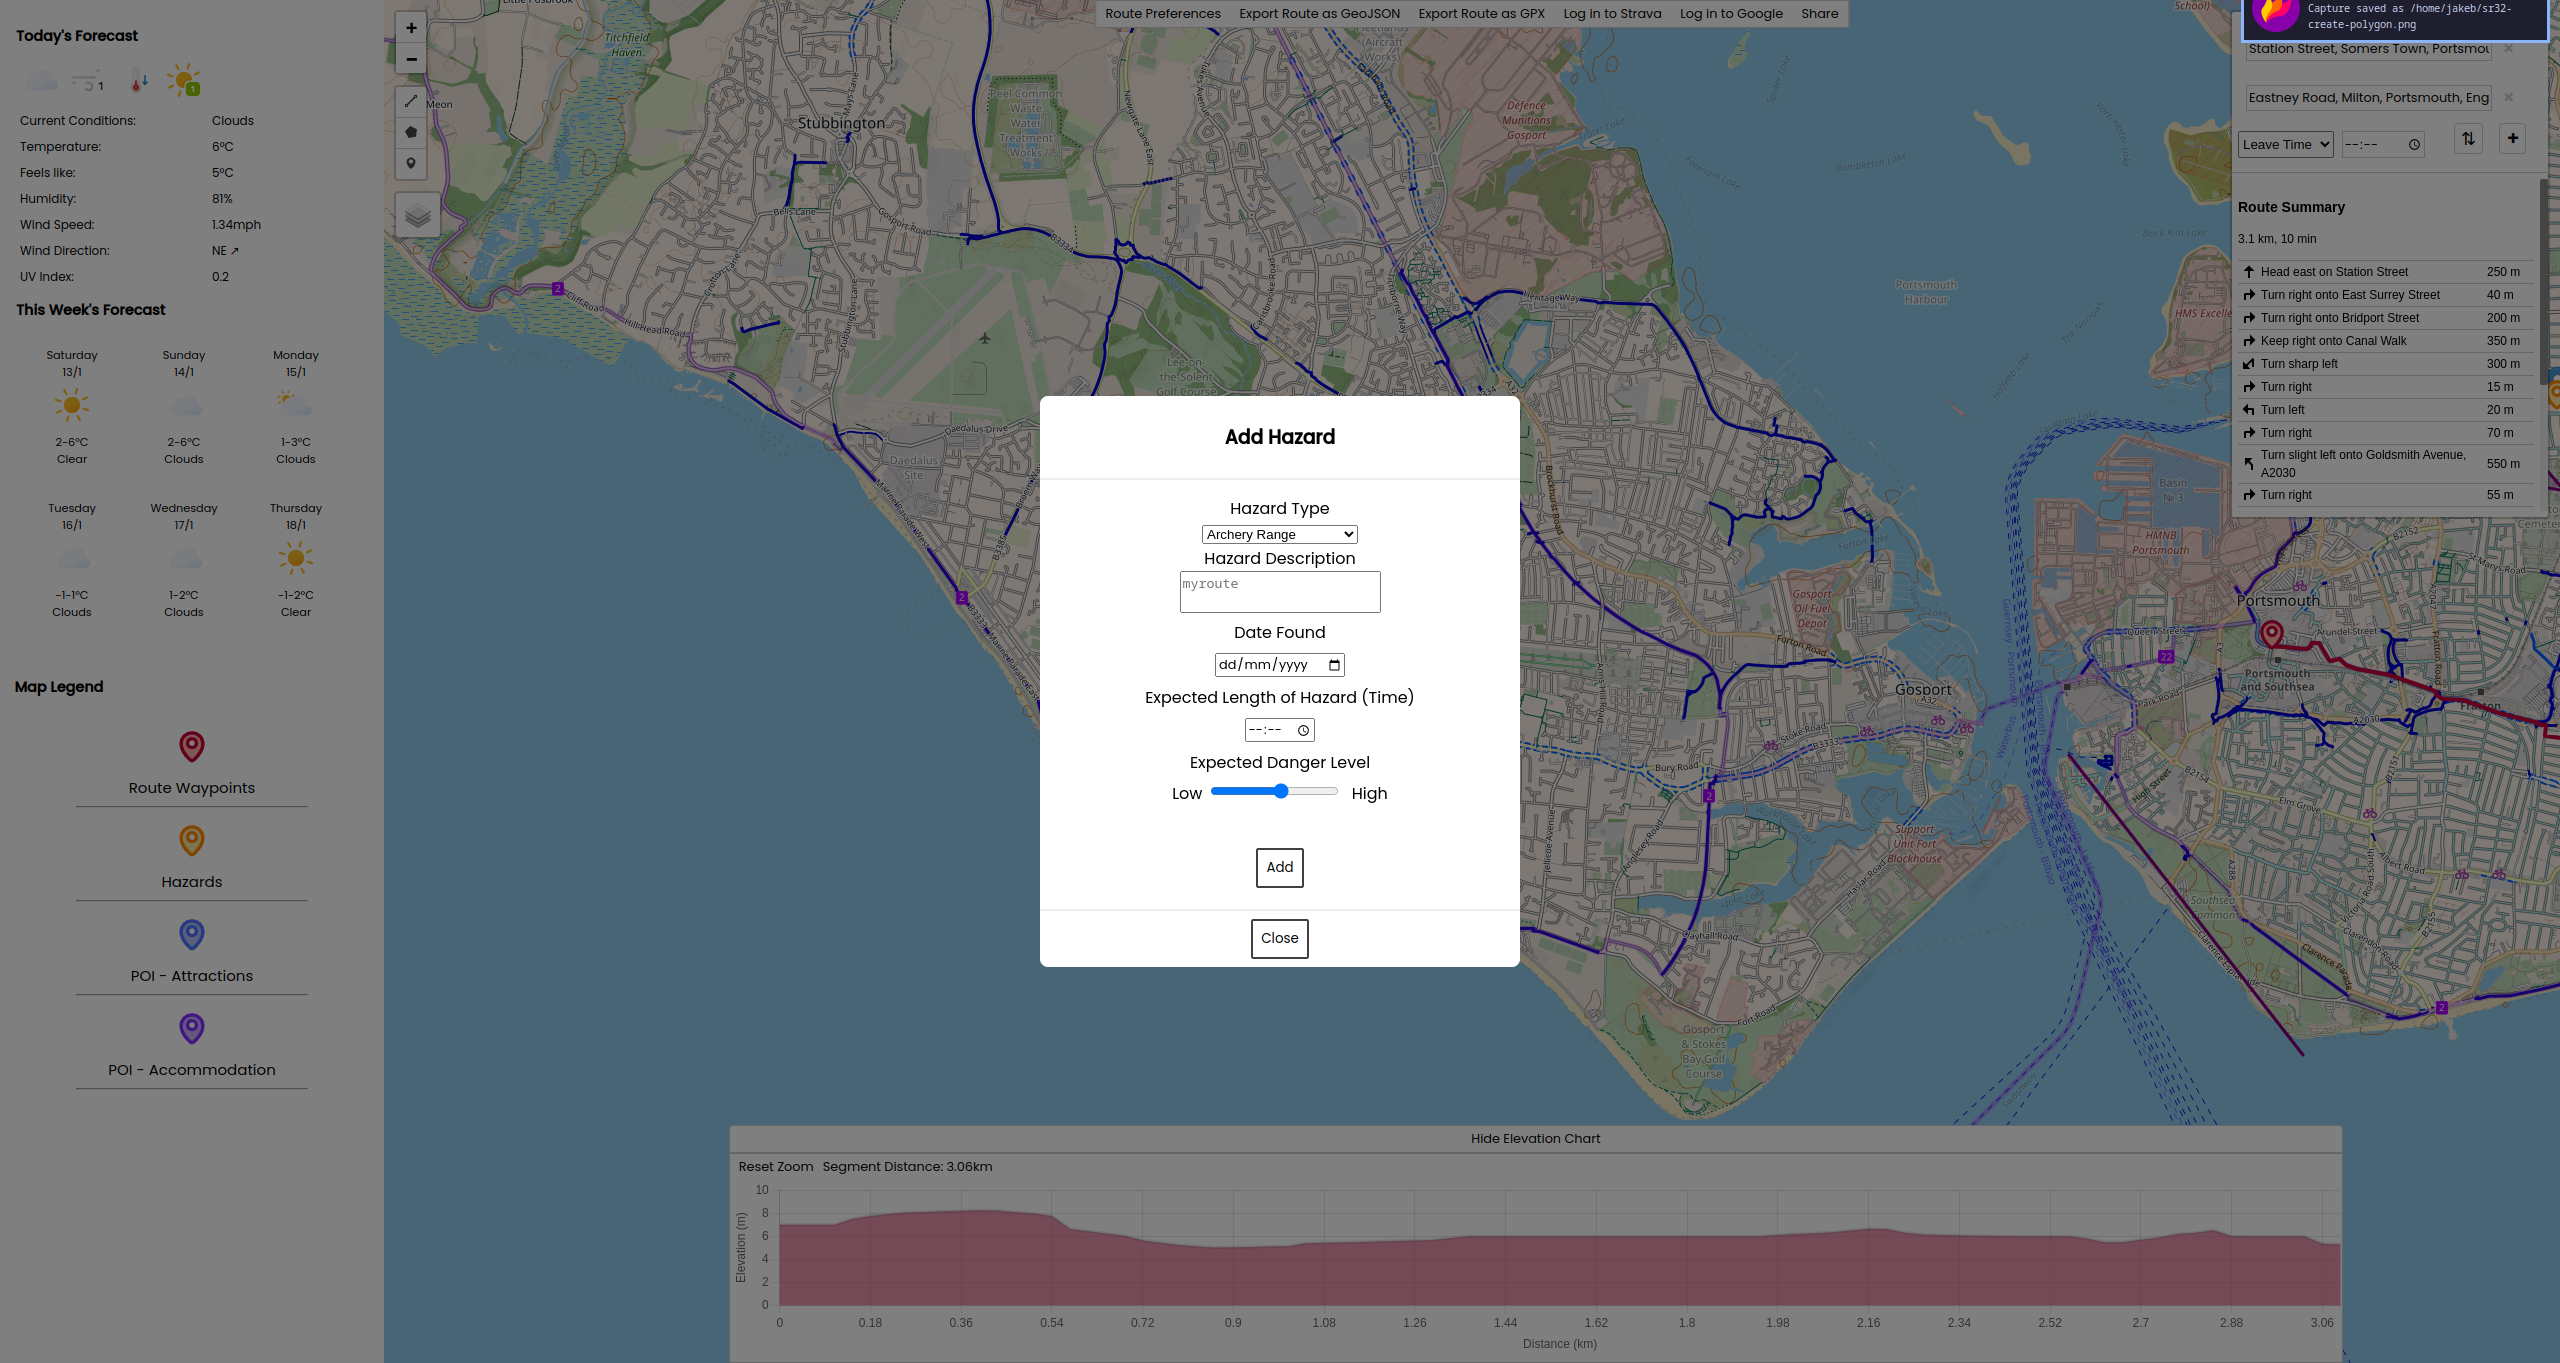
\includegraphics[width=425px]{figures/Progress Images/Iteration-2/SR32-37/sr32-add-hazard-point.png}
  \caption{Hazard Creation Modal}
  \label{fig:hazard-creation}
\end{figure}

\begin{figure}[!ht]
  \centering
  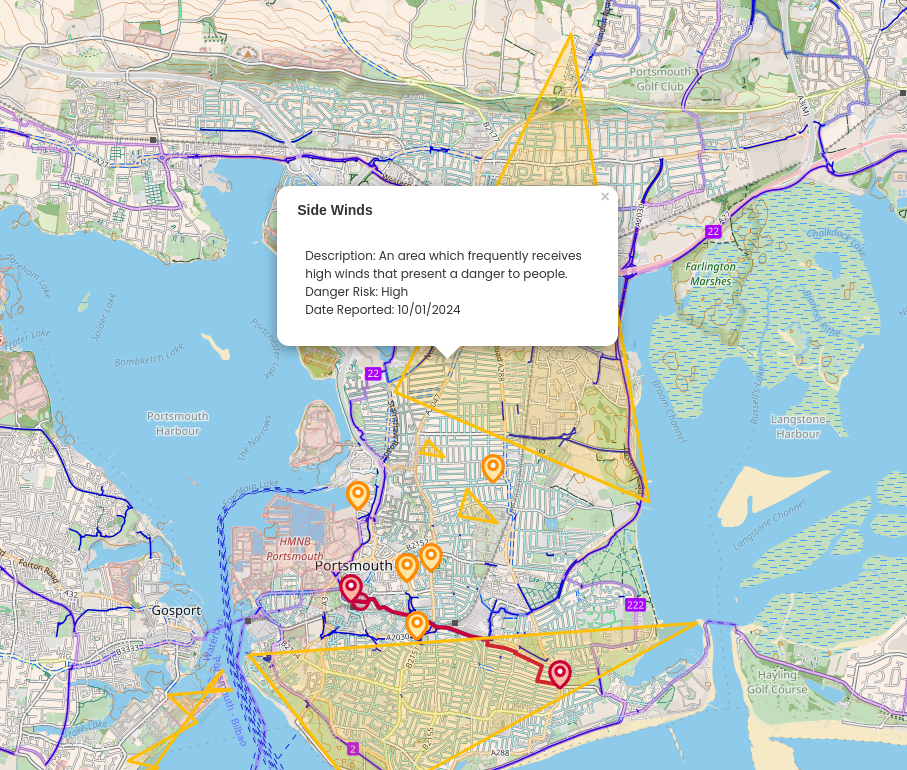
\includegraphics[width=300px]{figures/Progress Images/Iteration-2/SR32-37/sr32-hazard-popup.png}
  \caption{Hazard Map Layer}
  \label{fig:hazard-layer}
\end{figure}

\begin{figure}[!ht]
  \centering
  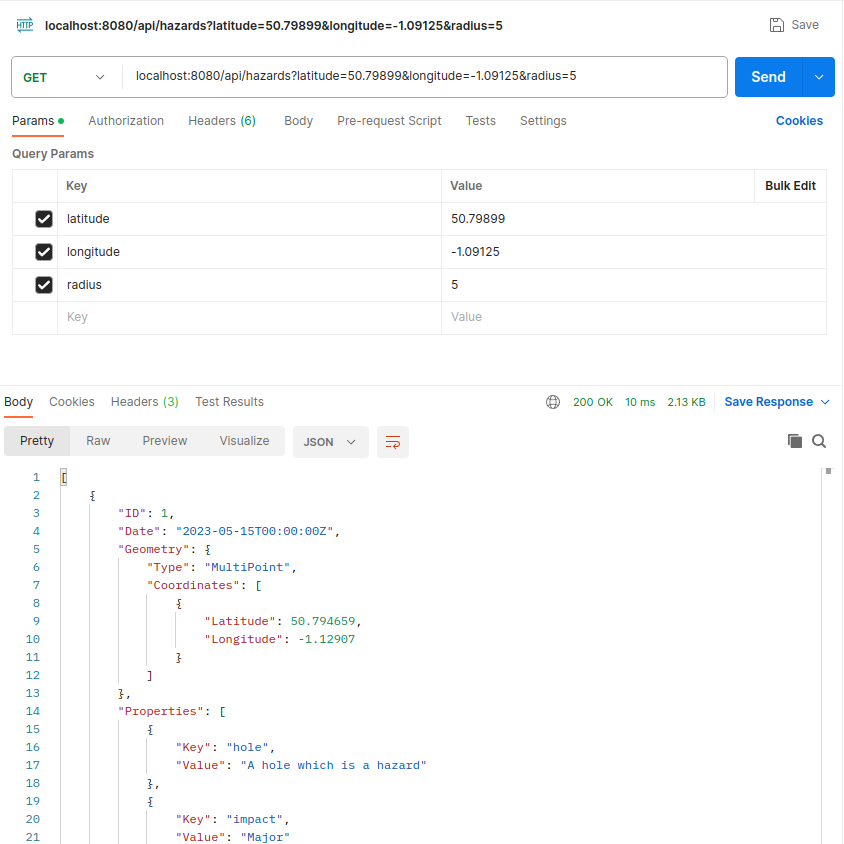
\includegraphics[width=425px]{figures/Progress Images/Iteration-2/SR32-37/SR32 - Basic API further developed.png}
  \caption{Hazard API Query}
  \label{fig:hazard-API}
\end{figure}

\subsection{Key Point-of-Interest (POI) Integration}
\label{iteration2:poi-integration}

The POI integration was the final feature of i2, where the user could view POI in their area retrieved from the Foursquare Places API (\cite{noauthor_places_nodate}). Two separate map layers were created similar to the hazard layer \see{iteration2:hazard-index}, one to display accommodation POI and another to display the attractions/leisure POI \see{fig:poi-layers}. The layer also allowed the user to click on each POI marker to view more information about the location, such as the name and address.

After the core POI layers were developed, two buttons were then added to each POI popup window. These were to allow a user to either route to or via the POI. If the user chose to route to, the last route waypoint would be updated to the POI's latitude and longitude. Whereas to route via, the route waypoints would initially be taken to find which route waypoint was closest to the POI, it would then be inserted into waypoints before the closest waypoint. The route would then be recalculated to include the POI as a waypoint \see{fig:poi-route}.

\begin{figure}[!ht]
  \centering
  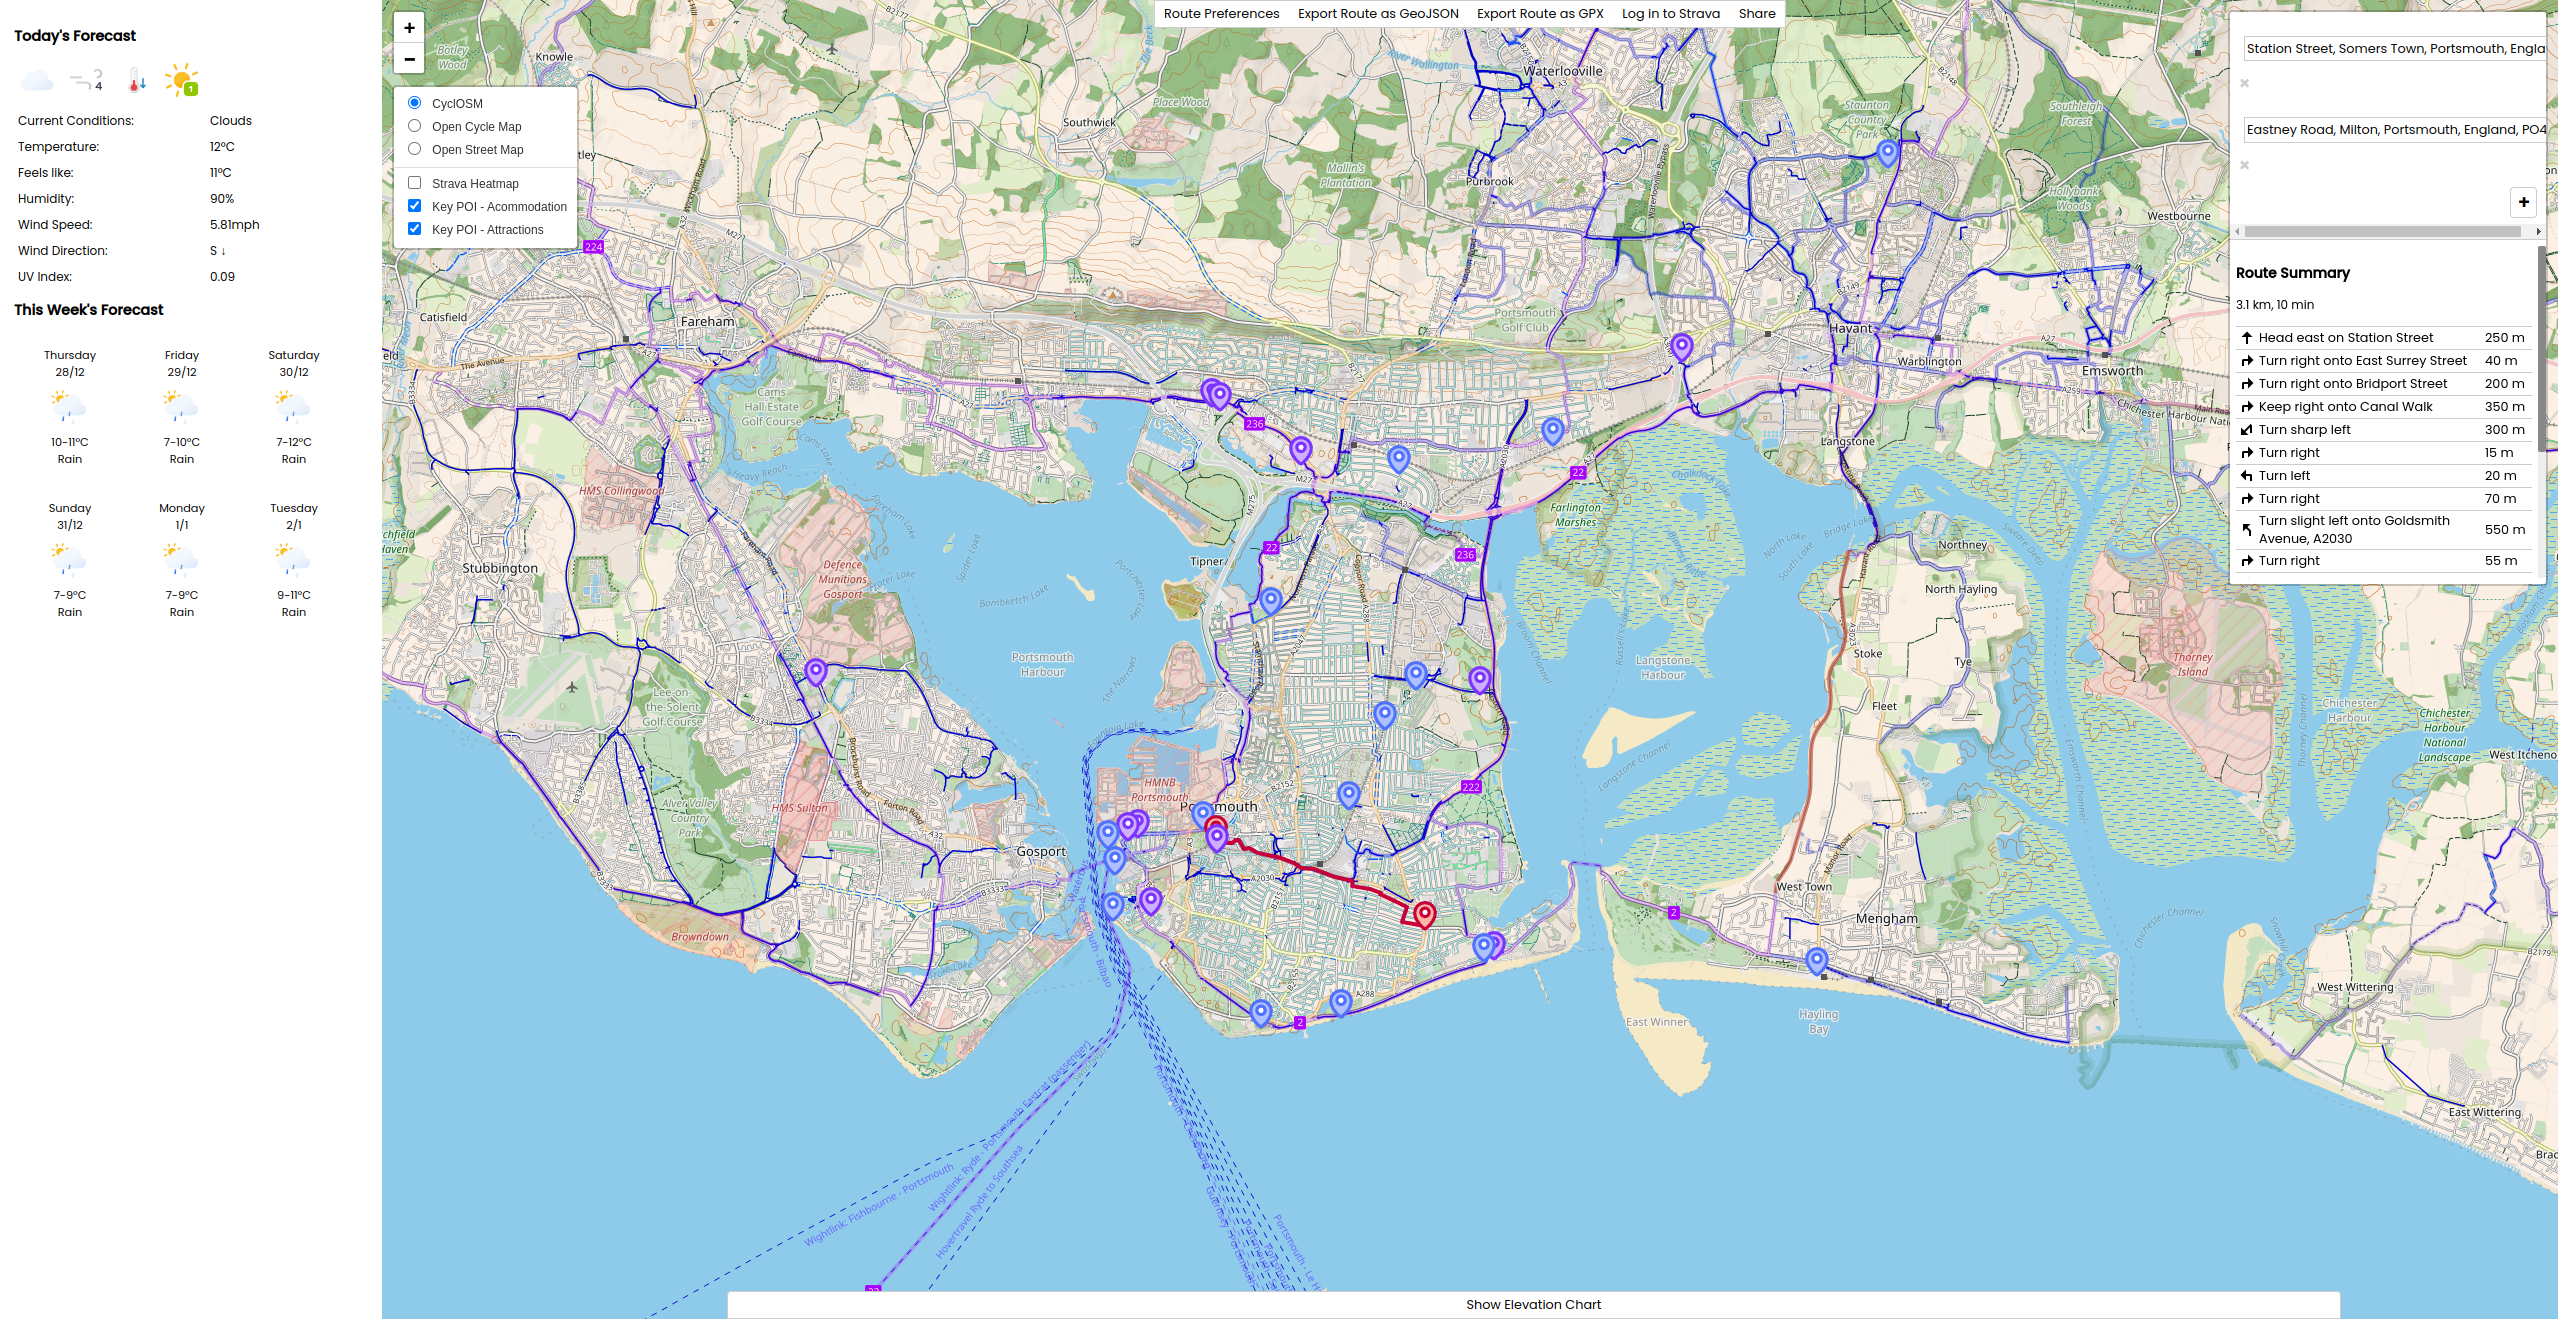
\includegraphics[width=425px]{figures/Progress Images/Iteration-2/SR40-45/SR40 - Attractions and Accommodation KeyPOI.png}
  \caption{Attractions and Accommodation Layers}
  \label{fig:poi-layers}
\end{figure}

\begin{figure}[!ht]
  \centering
  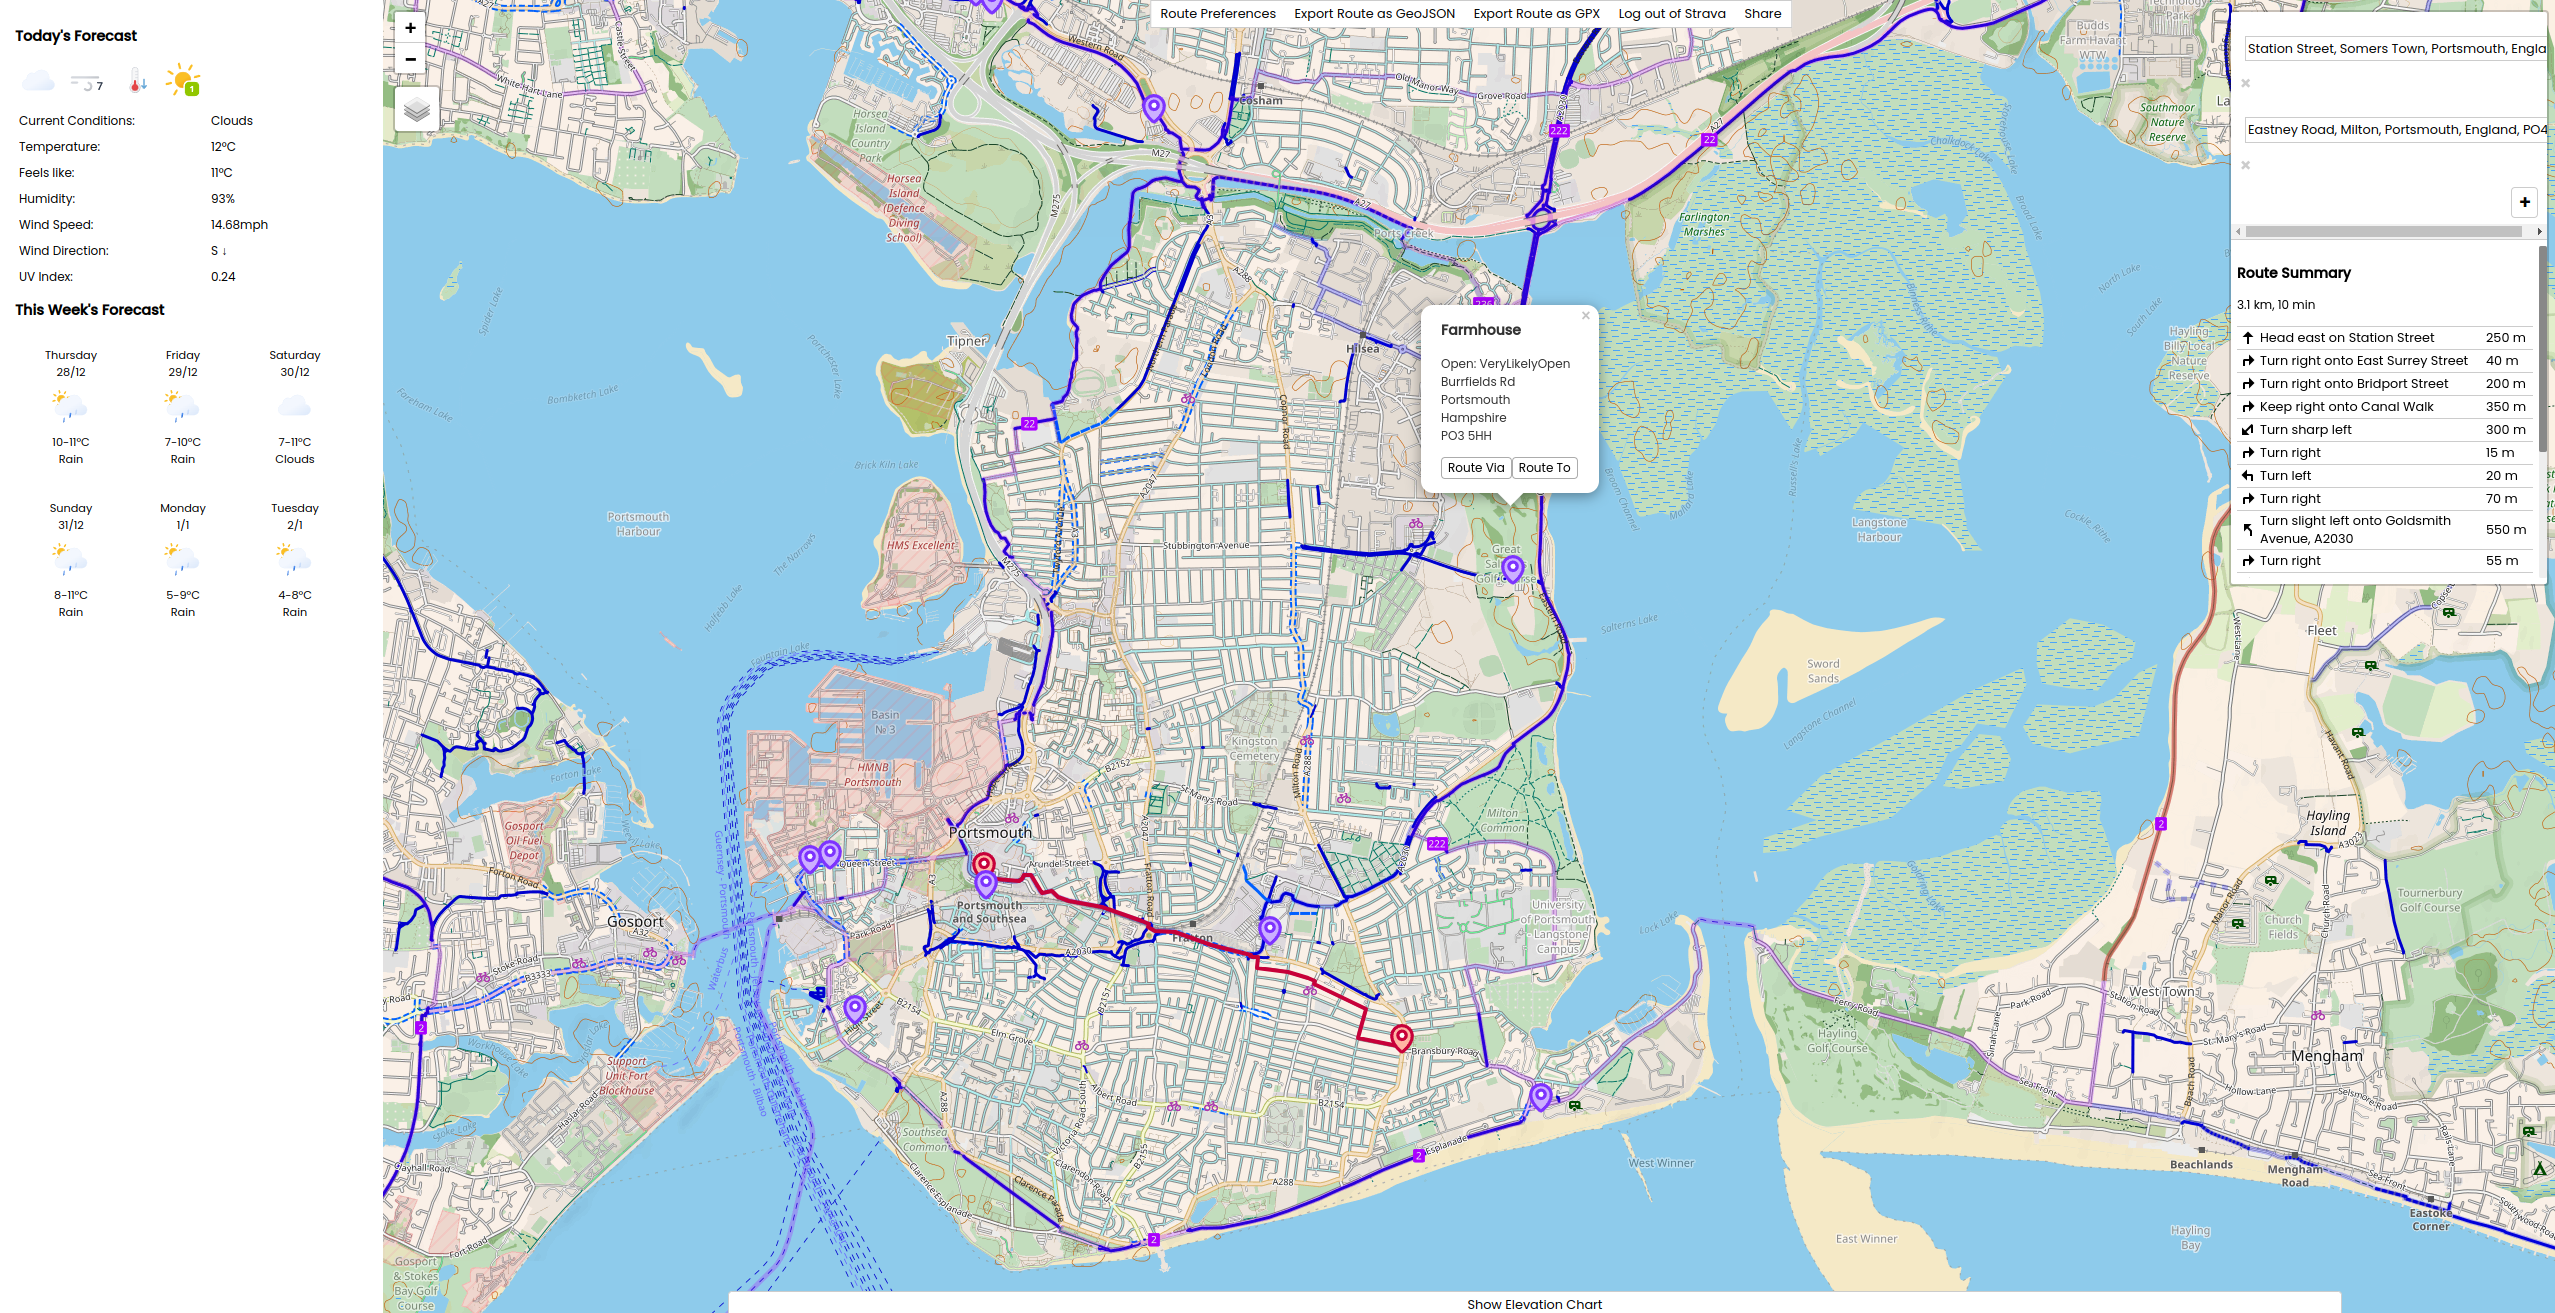
\includegraphics[width=425px]{figures/Progress Images/Iteration-2/SR40-45/SR45 - Route ToVia POI.png}
  \caption{Route To/Via POI}
  \label{fig:poi-route}
\end{figure}

\subsection{Main Challenges}
\label{iteration2:main-challenges}

The main challenges for i2 resided in setting up the SQL queries to handle the hazard data requests as well as oauth authentication with the Strava API.

The INSERT hazard query was the most complex. The PLpgSQL language was used to create a function to handle this logic as loops were required when inserting multiple PostGIS Point data types (coordinates) for each hazard. A loop was required to insert the properties for each hazard, where each hazard could have one or more. The function was then called from the API endpoint, passing the json string input directly into the PLpgSQL function.

The Strava API was also challenging as it was required to implement oAuth 2.0 manually to authorise the application to access the user's account. The API documentation was relatively clear on how to implement this process, however, having not manually implemented oAuth before, without using libraries such as Auth0, it was a steep learning curve. This experience proved useful later when implementing oAuth 1.0 for use with the Garmin Connect API \see{iteration3:garmin-integration}.

\clearpage
\section{Iteration 3 - Round Trip, Route Import and Garmin Integration}
\label{implementation:iteration3}

Finally, i3 included the remainder of the critical and desired requirements. These included round-trip routing, route import, Garmin Connect integration and social media sharing. There were only a few requirements that were not implemented due to time constraints, these were the lowest priority requirements and were not critical to the artefact's functionality.

\subsection{Round Trip Routing}
\label{iteration3:round-trip}

The ORS API was implemented shortly after it was found that OSRM didn't support round-trip routing, only A to B routing \see{iteration1:basic-routing}. The new API was implemented towards the end of i1 ahead of knowing the requirements for i3. 

To implement round-trip, the library used for using ORS with Leaflet Routing Machine (\cite{noauthor_gegewebleaflet-routing-machine-openroute_2020}) was customised to fit the artefact's needs. A fork was created to allow the round-trip feature to be used with the library. This fork allowed for only one waypoint to act as an input to trigger the API call for round-trip routing. The API call would then return a route in the same format as an A to B route, with the start and end being the same point. The route was then drawn on the map and the elevation chart was updated. \see{fig:round-trip}.

Once the updates were made to the forked library, the other functionalities of the artefact worked seamlessly in both the standard A to B and the round-trip mode. The only minor change required was to track the mode in which the user last left the artefact in LocalStorage. This then ensured that when the user returned and chose to load their previous route, the artefact would know which mode to load the route on.

\begin{figure}[!ht]
  \centering
  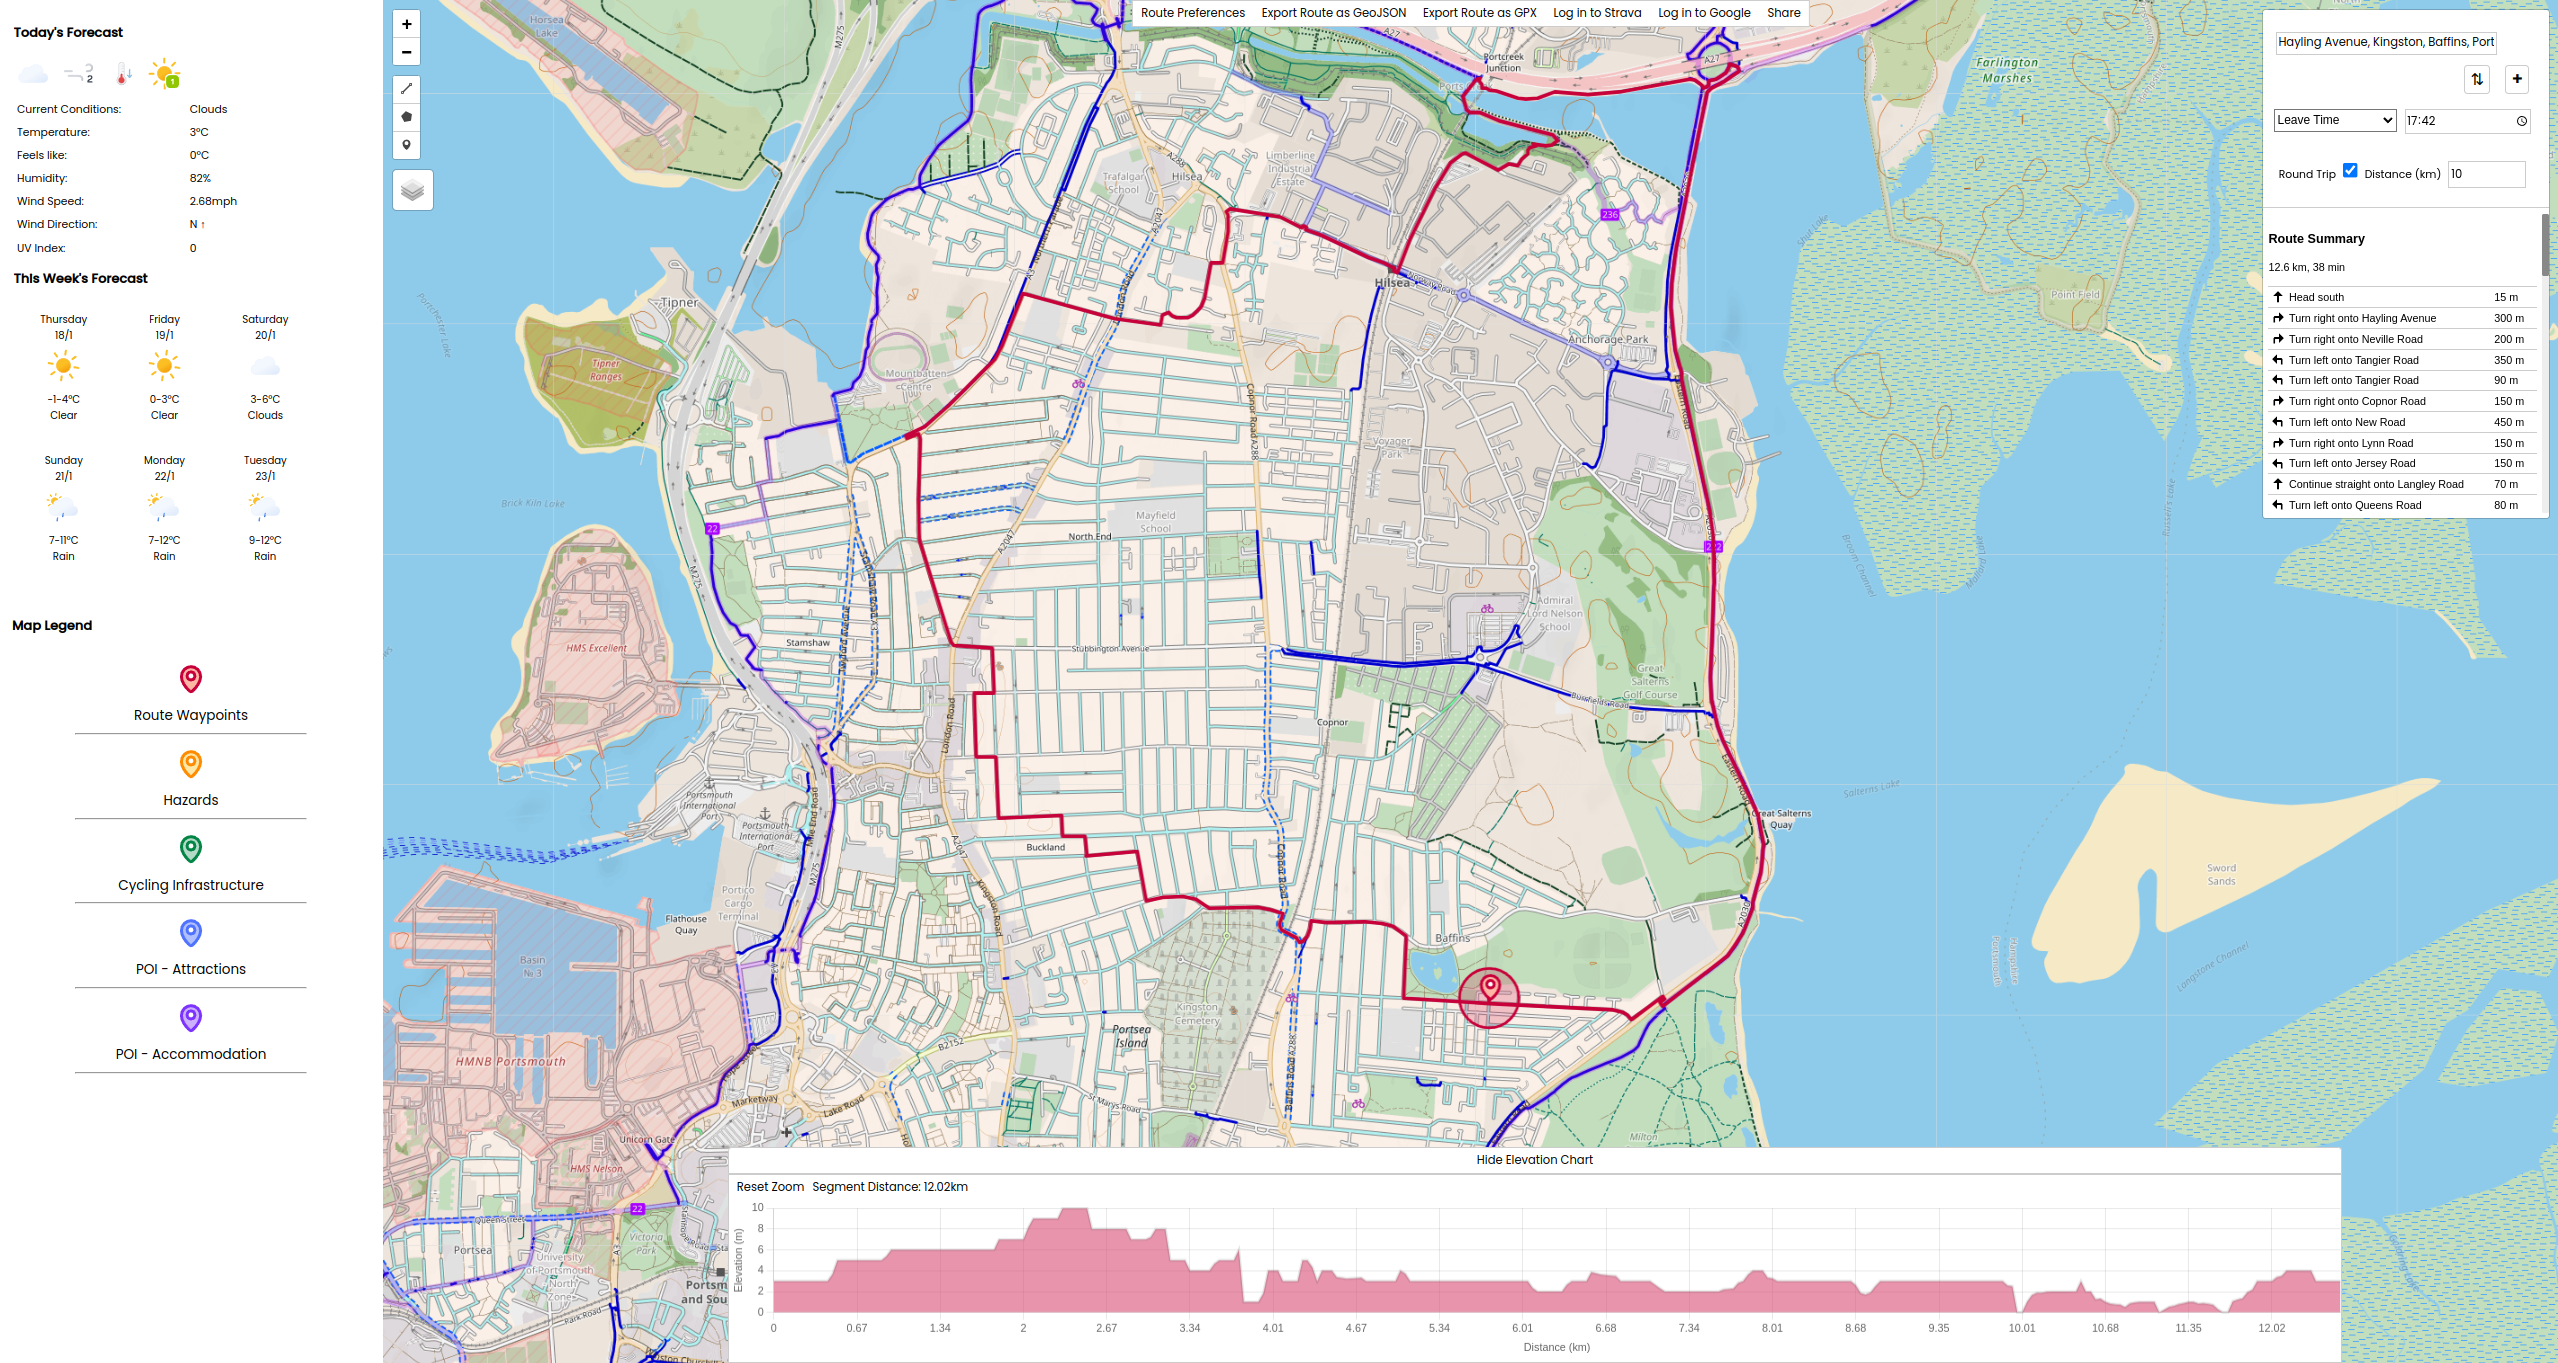
\includegraphics[width=425px]{figures/Progress Images/Iteration-3/SR11/SR11- Round Trip functionality working.png}
  \caption{Round Trip Route}
  \label{fig:round-trip}
\end{figure}

\subsection{Route Import}
\label{iteration3:route-import}

Route imports were a vital feature to enable route sharing across many applications supporting the same standards. The GPX and GeoJSON file formats were chosen to be supported as they are the most common file formats used for route sharing and were already used for exporting routes from the artefact. Adding such a minor feature would enable the artefact to manually import routes from other applications, such as Strava, Komoot and RideWithGPS.

To interpret the GPX string, the \texttt{DOMParser} was used to parse the string into an XML document. The XML document was then traversed to find the route's latitude and longitude points, which were then stored in an array of coordinates. This array was then stored in a state variable called 'waypoints'. For GeoJSON, the \texttt{JSON.parse} method was used to parse the string, then the coordinates were extracted and stored in the same way as the coordinates in the GPX \see{fig:gpx-import}.

\label{fig:route-import}
\begin{figure}[!ht]
  \centering
  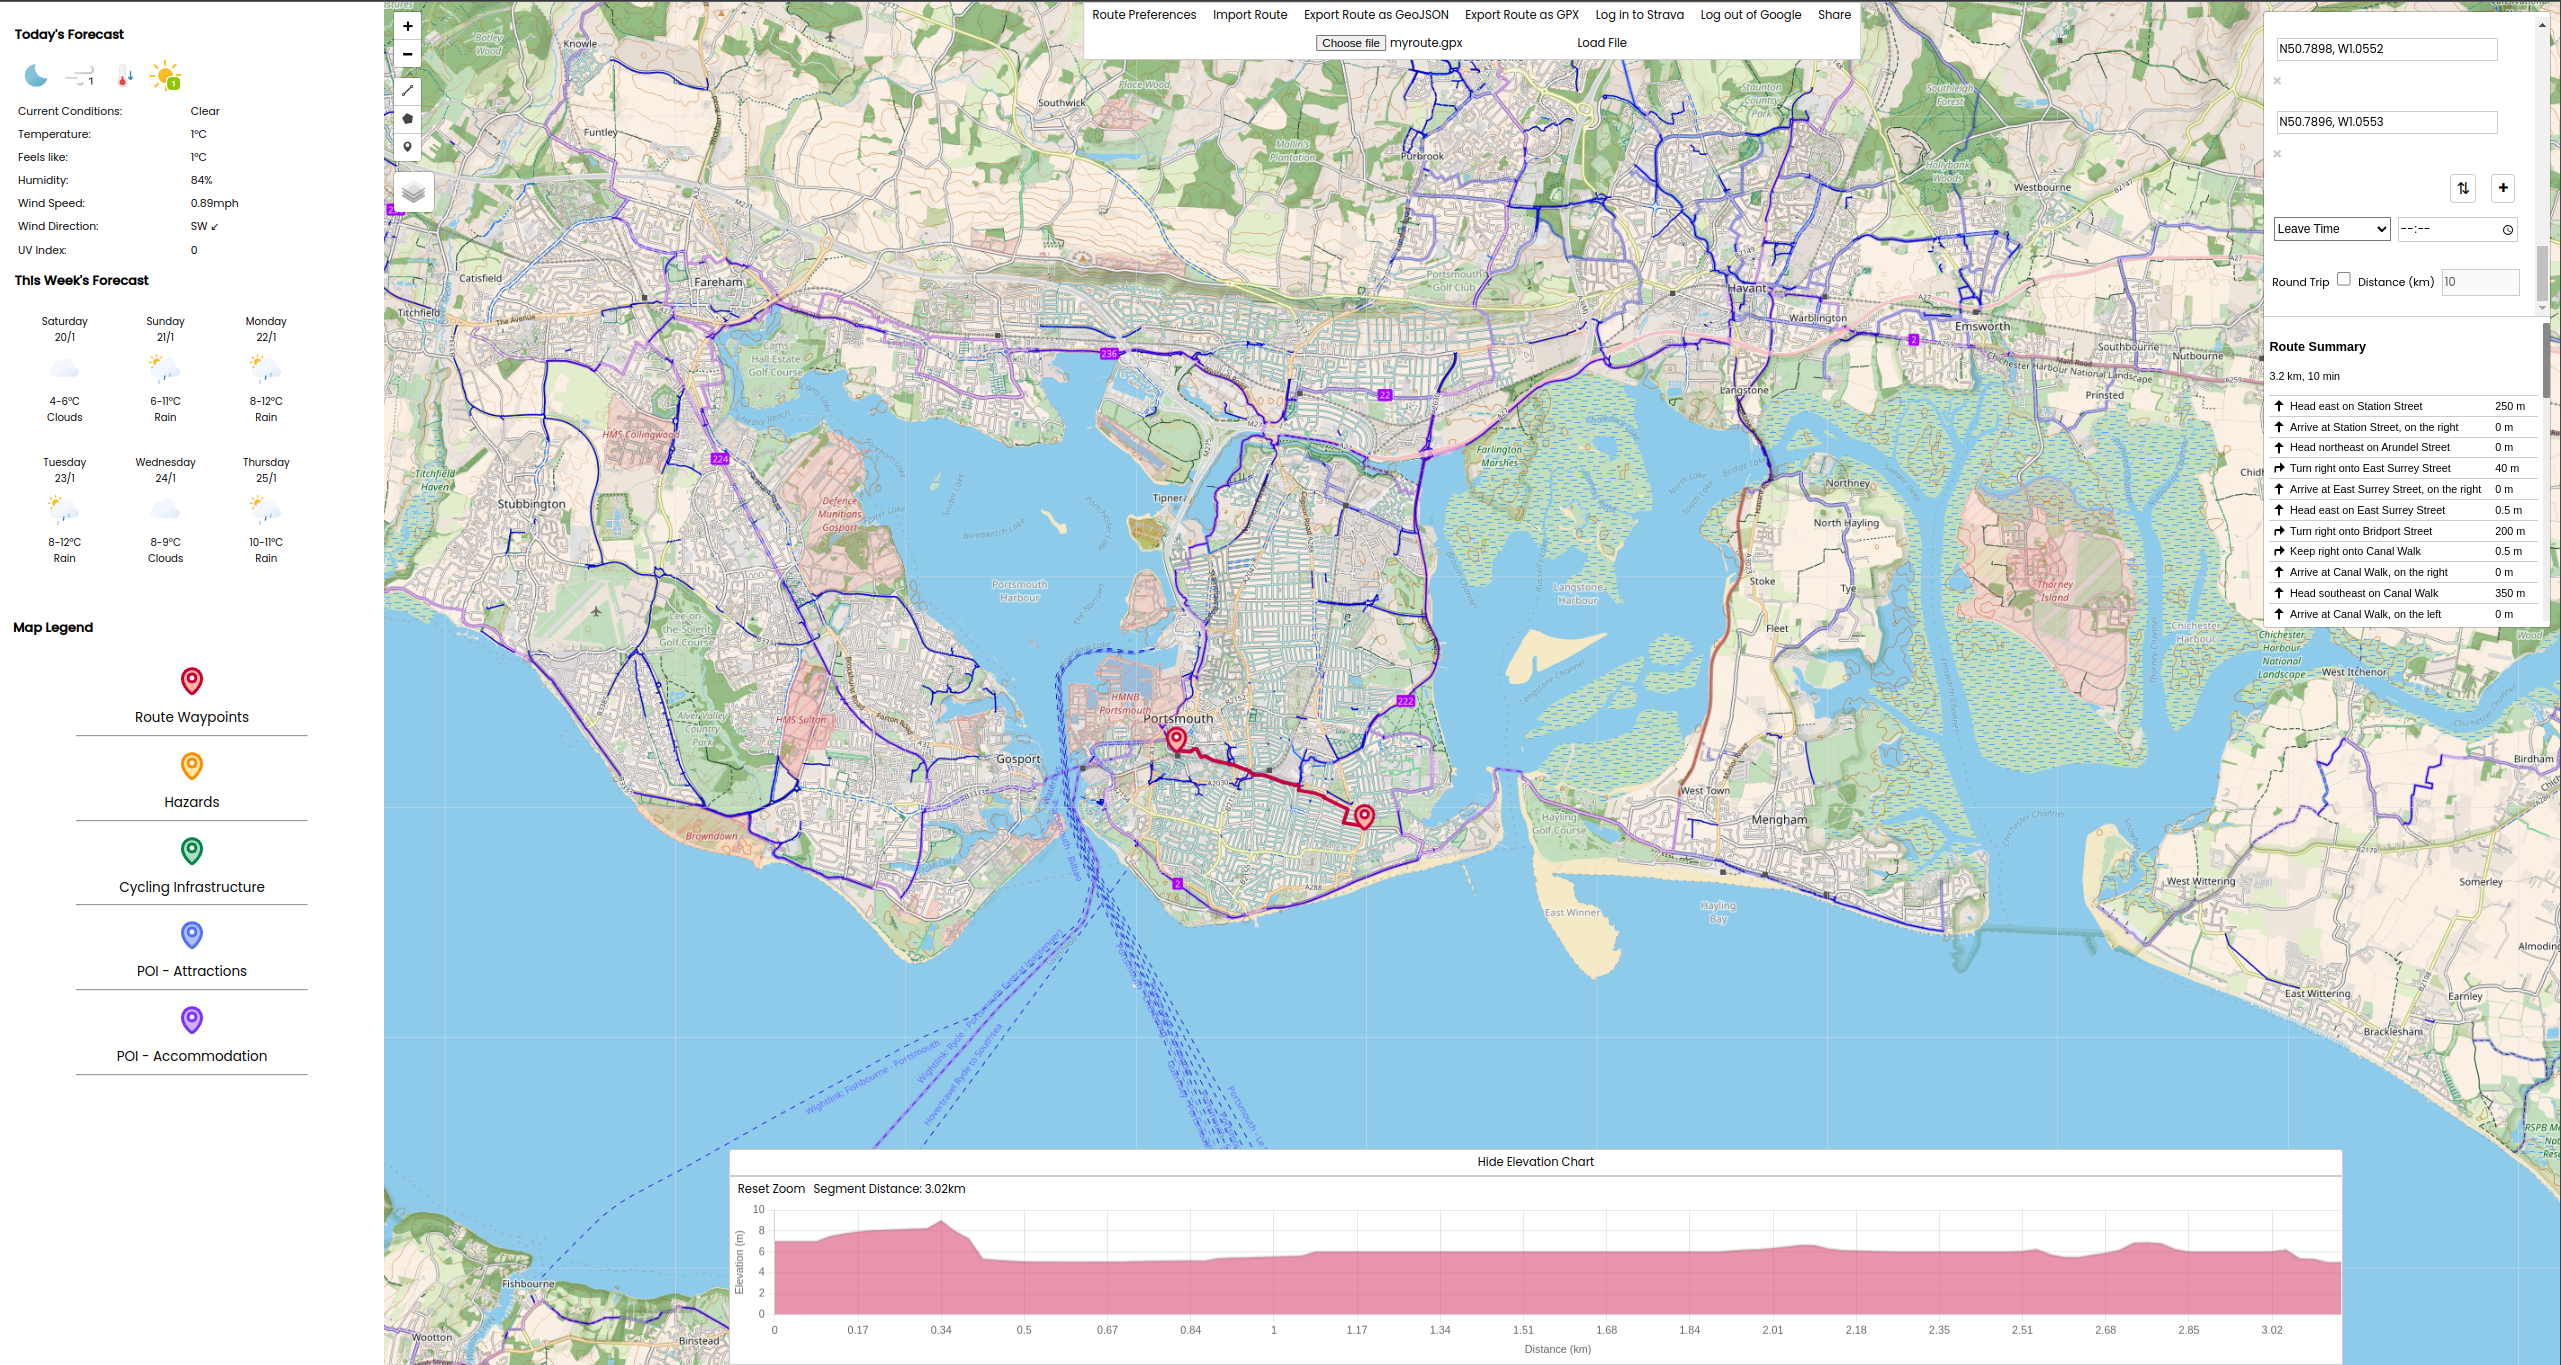
\includegraphics[width=425px]{figures/Progress Images/Iteration-3/SR48-49/SR48-Import GPX.png}
  \caption{Import GPX Route}
  \label{fig:gpx-import}
\end{figure}

\subsection{Garmin Connect Integration}
\label{iteration3:garmin-integration}

To integrate with the Garmin Connect API, the oAuth 1.0 protocol was implemented to allow the artefact to access the user's Garmin Connect account. The oAuth 1.0 protocol was implemented manually, as the Garmin Connect API documentation was clear on the oAuth process, having implemented oAuth 2.0 for Strava \see{iteration2:sharing-route}, the process was more understandable.

Once authentication had been completed, the create route endpoint was set up to handle the POST request from the front end. The endpoint required the oAuth token, secret, the route details as a route JSON string. The fetch API was then called to make the post request to the backend which would pass the route to the Garmin API to be uploaded. The route was then stored as a course in the user's Garmin Connect account, where it could be accessed from the Garmin Connect website or app \see{fig:garmin-connect}. 

\label{fig:garmin-connect}
\begin{figure}[!ht]
  \centering
  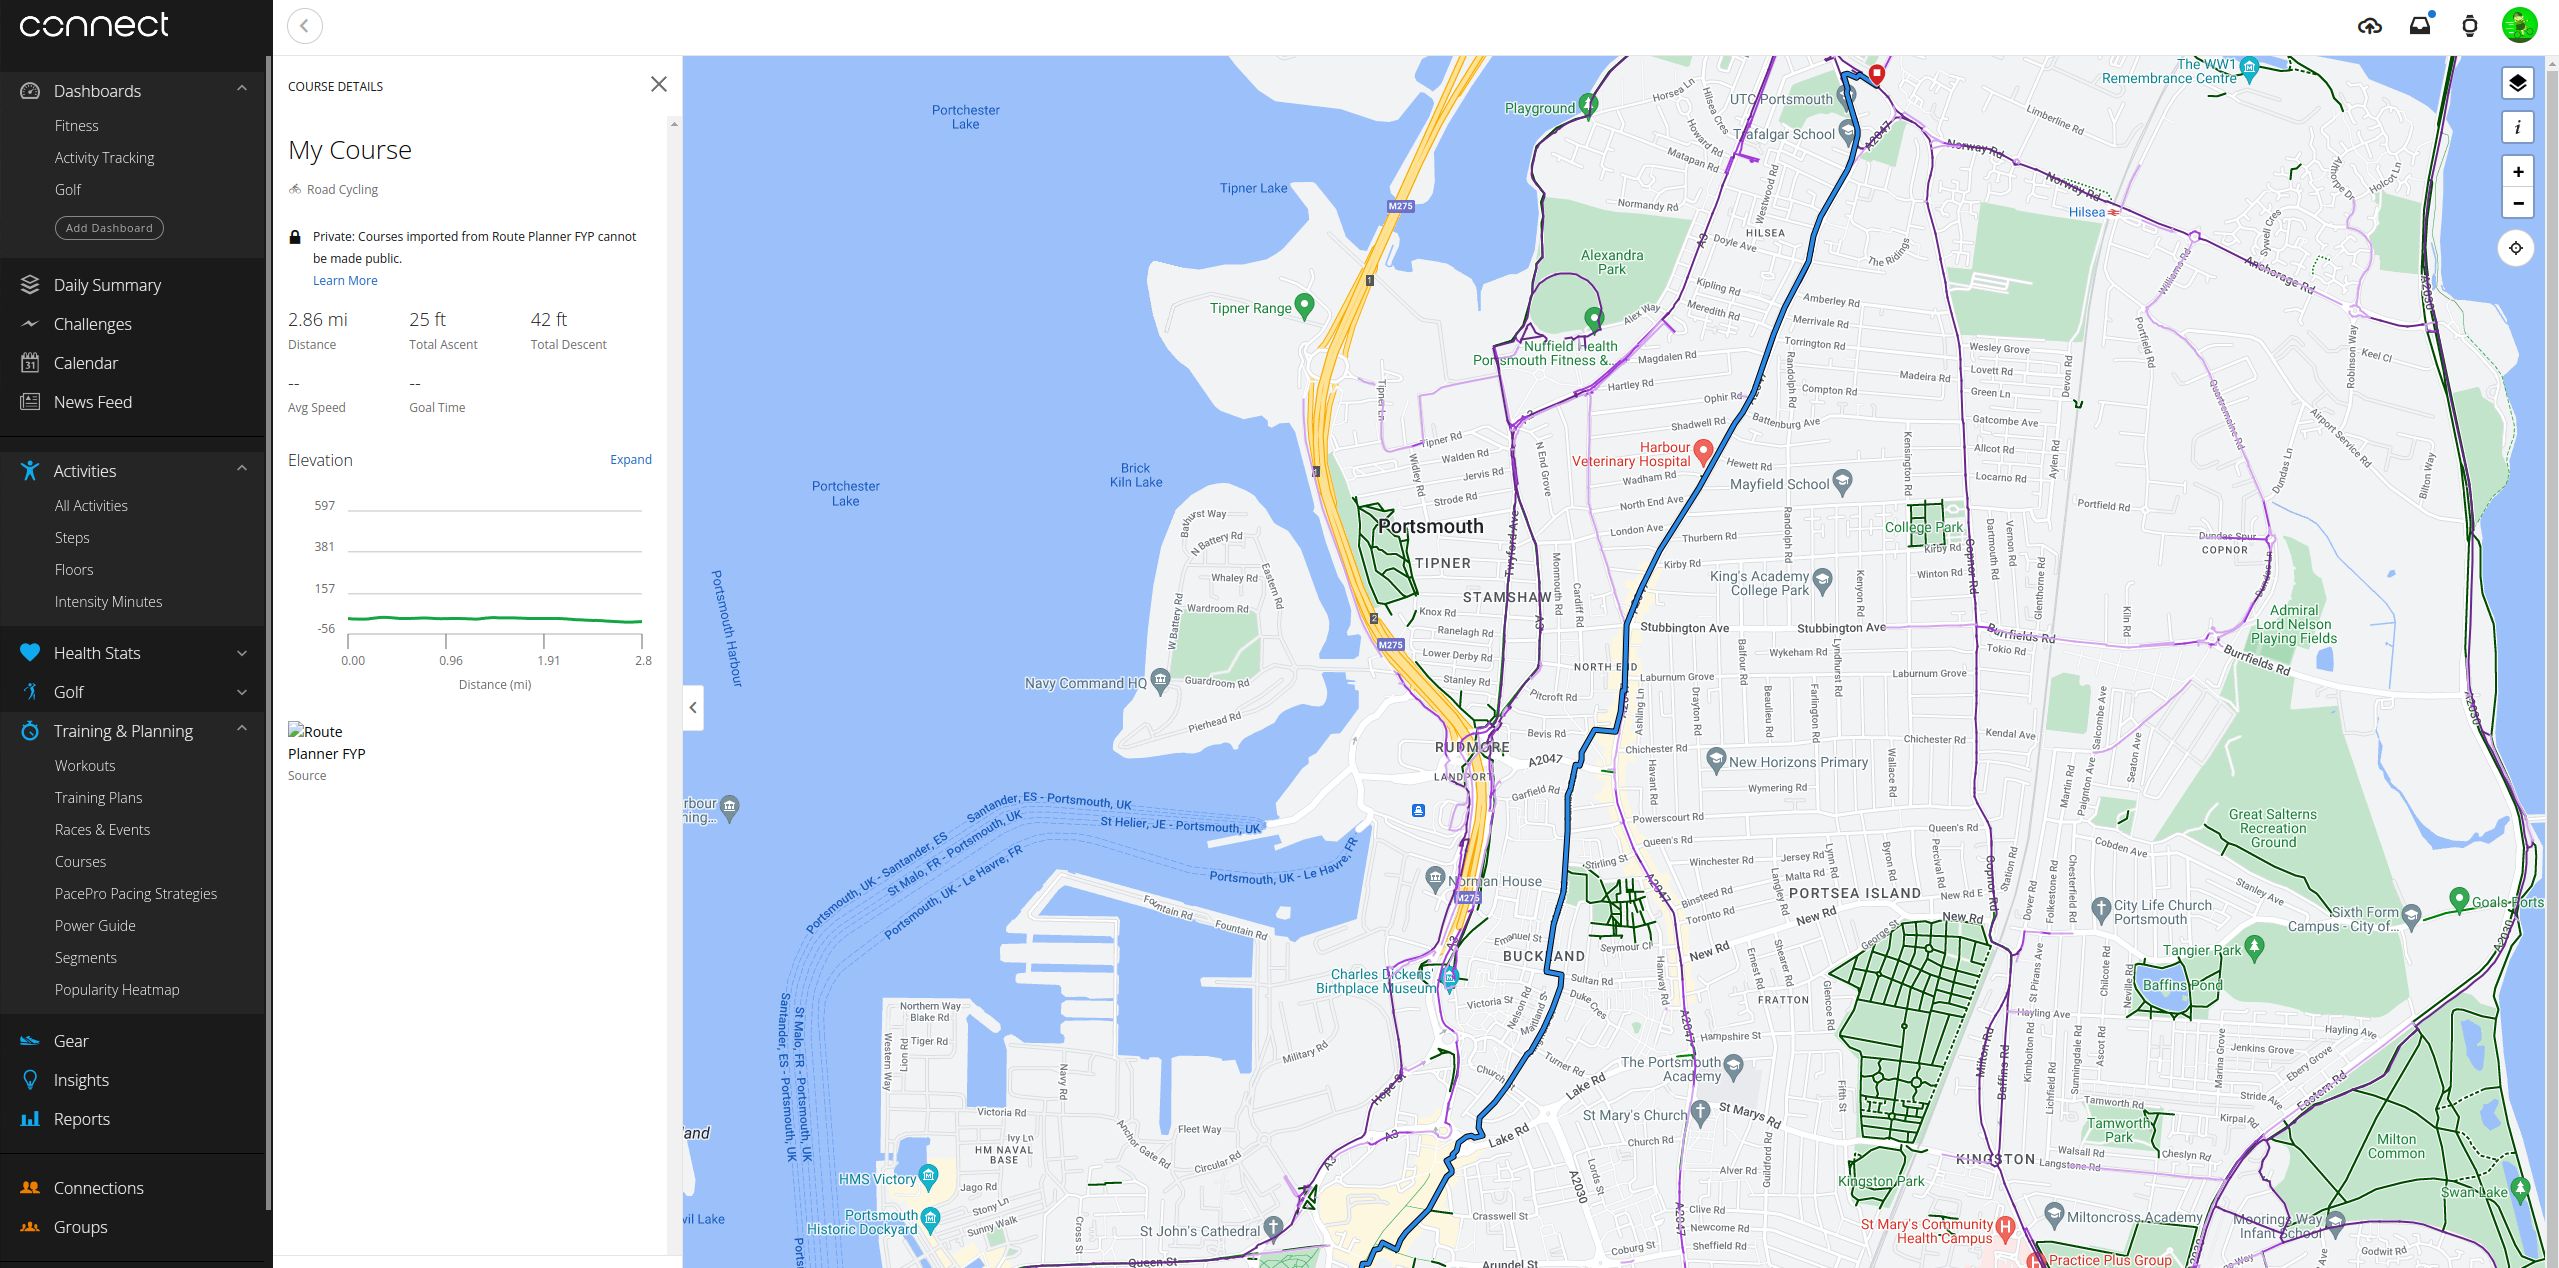
\includegraphics[width=425px]{figures/Progress Images/Iteration-3/SR50/SR50 - Garmin Connect App Course Viewer.png}
  \caption{Garmin Connect Successfully Uploaded Route}
\end{figure}

\subsection{Social Media Sharing}
\label{iteration3:social-sharing}

The final feature to be implemented was sharing with Facebook, X(Twitter), and Reddit to allow an image of the route to be shared to the user's social media account. The route image was generated with the leaflet screenshotter library (\cite{noauthor_leaflet-simple-map-screenshoter_2022}). The furthest two coordinates were calculated using the Euclidian distance formula \see{iteration3:euclidian-distance}, then the map's bounds were set to fit the two points and a map screenshot was taken as a base64 string. This string was then passed to the respective social media API to be shared to the user's account \see{fig:facebook-share}.

\begin{equation}
  \label{iteration3:euclidian-distance}
  distance = \sqrt{(x_2 - x_1)^2 + (y_2 - y_1)^2}
\end{equation}
Where $x_1$ and $y_1$ are the latitude and longitude of the start point, and $x_2$ and $y_2$ are the latitude and longitude of the end point.

\begin{figure}[!ht]
  \centering
  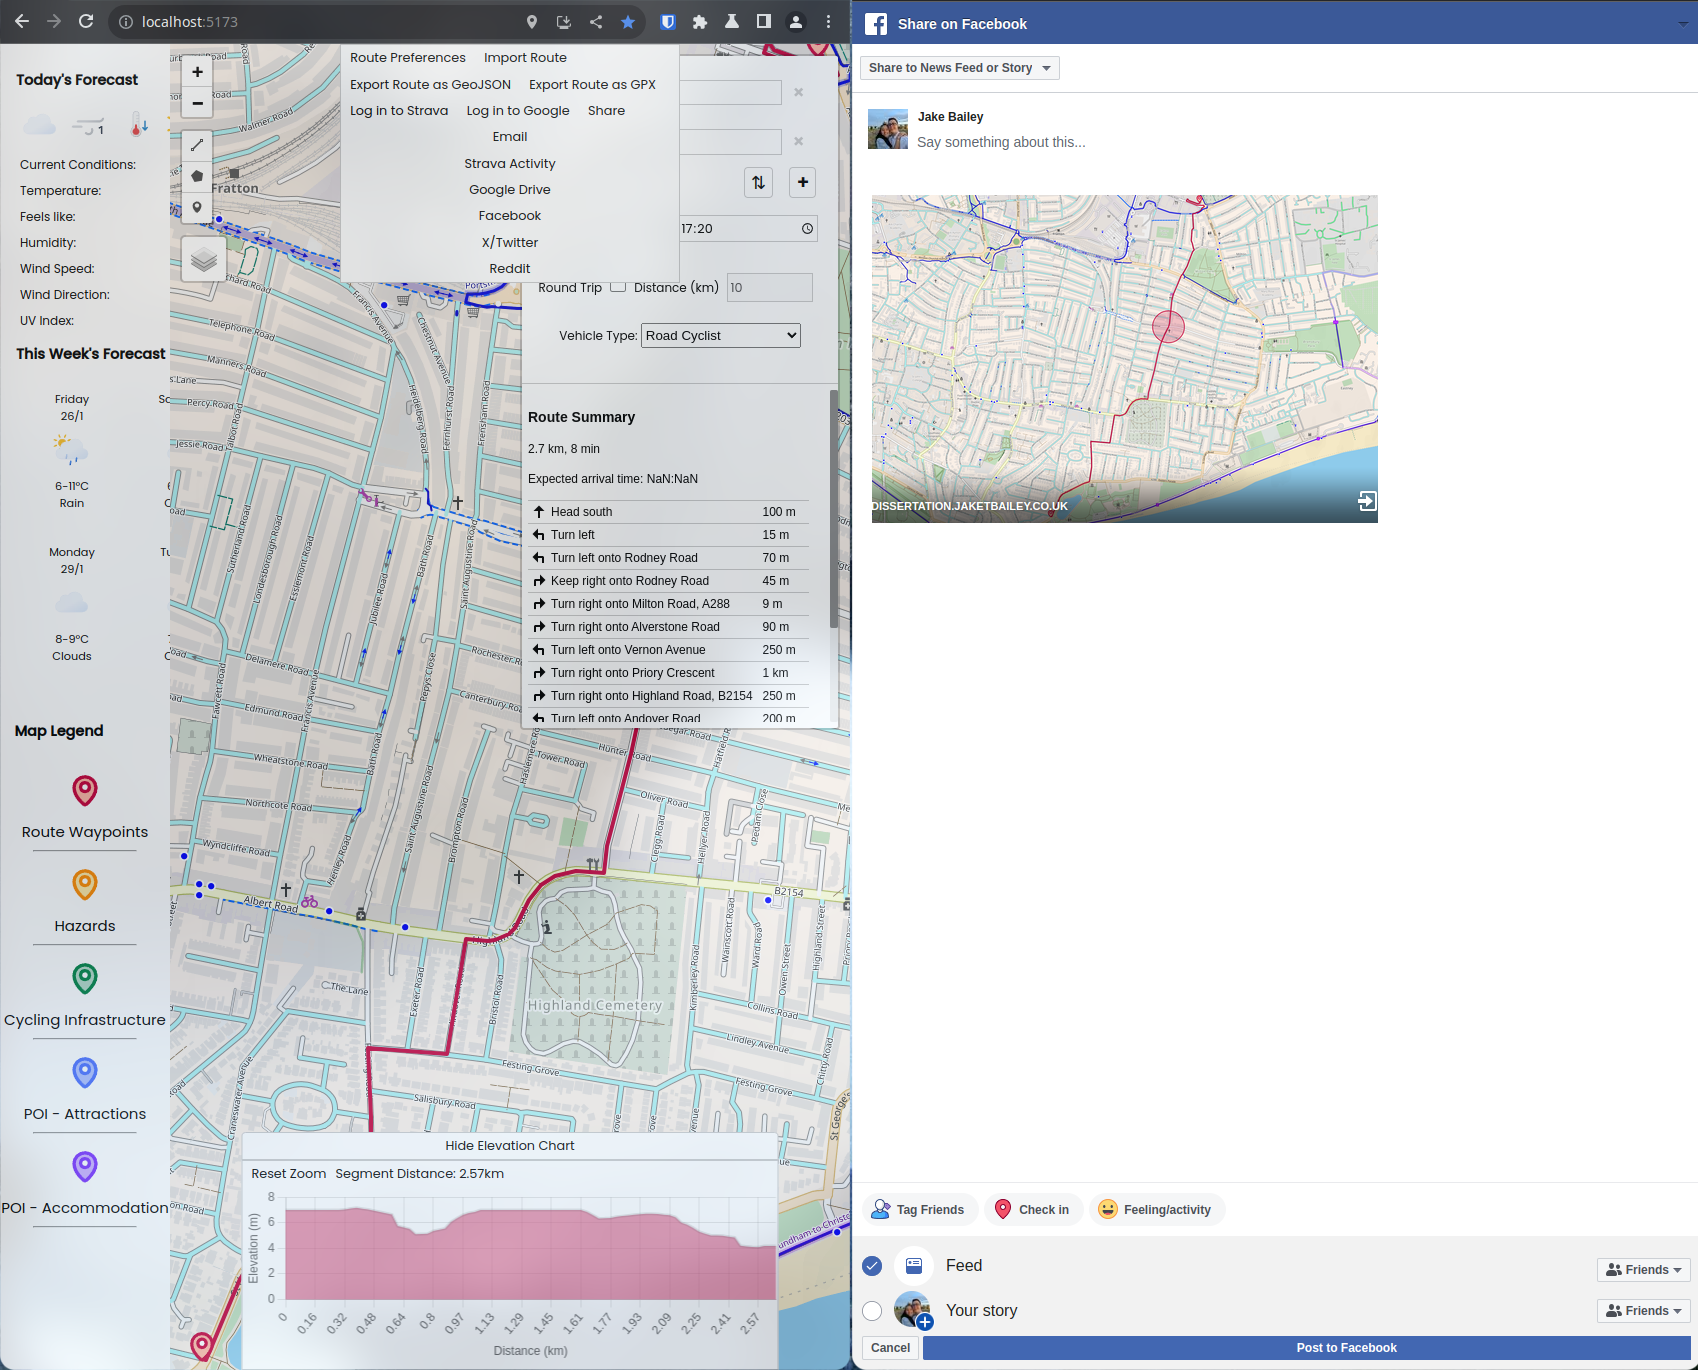
\includegraphics[width=425px]{figures/Progress Images/Iteration-3/SR51/SR51-Share to Facebook.png}
  \caption{Share to Facebook}
  \label{fig:facebook-share}
\end{figure}

\subsection{Main Challenges}
\label{iteration3:main-challenges}

The main challenge of i3 was the oAuth 1.0 protocol for the Garmin Connect API. Despite having implemented oAuth 2.0 for Strava \see{iteration2:sharing-route}, Garmin did use an alternative protocol. The logic used for the Strava oAuth process was not transferable, therefore it had to be implemented from scratch. Minor issues with React were also found where in developer mode, the artefact would re-render twice, leading to the user-independent token being changed twice, causing issues with the oAuth process. This was resolved through thorough debugging, ensuring correct use of the useEffect and testing in production mode.